% !Mode:: "TeX:UTF-8" 

\BiChapter{基于X-means聚类的克隆代码演化特征分析}
{Analyzing Clone Evolutionary Characteristic Based on X-means Clustering}

\BiSection{引言}
{Introduction}

研究表明软件中存在大量的克隆代码,在软件随着时间进行演化的过程中,克隆代码也会随着软件系统进行演化,将克隆代码的这一现象称为克隆代码演化。在大量克隆代码及其演化过程中,必然存在着一些隐含的信息可以揭示克隆演化规律,本文将之称为克隆代码演化特征。克隆演化特征不仅可以帮助软件开发人员理解系统中存在的克隆代码,还可以向软件开发人员提供一些如何维护克隆代码的建议。但遗憾的是,当前研究中对克隆演化特征的研究不够充分,缺乏客观且全面的克隆演化特征分析方法。因此,如何分析并获取克隆代码演化特征是一个值得研究的问题。

为帮助程序开发人员获得克隆代码演化特征,本章在提取克隆代码的属性特征的基础上,使用机器学习中的聚类方法挖掘克隆代码的演化特征,并验证了克隆代码的一致性维护的必要性。首先,通过映射相邻版本的克隆代码,构建软件系统的克隆家系。然后,从克隆片段、克隆组和克隆家系三个不同的角度描述克隆代码及其演化过程,并提取不同属性值表示克隆代码及其演化过程。最后,根据所提取的属性值生成相应的聚类向量,使用聚类方法挖掘和分析克隆代码的演化特征。在开源系统ArgoUML和jEdit上进行了实证研究,结果表明在演化过程中大部分克隆代码是稳定的,但也存在一定数量发生变化的克隆代码;且在发生变化的克隆代码中,大部分是发生一致性变化的克隆代码。因此,建议程序开发人员关注发生变化的克隆代码并对其进行一致性维护,为本文后续的克隆代码一致性维护需求预测研究奠定了基础。

\BiSection{克隆代码演化特征分析}
{Analyzing Clone Evolutionary Characteristic}

\BiSubsection{现有研究存在的问题}
{Problems in Current Research}

为描述克隆代码随着软件的演化过程,Kim等人提出了克隆家系模型\cite{kim2005empirical},并引发了对克隆代码演化以及演化规律的研究,例如克隆寿命、克隆稳定性与一致性变化等研究(如表~\ref{characteristic}~所示)。

在克隆代码随着软件演化的过程中,克隆代码会长时间的存在于系统中。研究人员通过对比克隆和非克隆代码,发现克隆代码比非克隆代码的寿命更长\cite{krinke2011cloned},且克隆代码的存在时间往往都会超过一年\cite{bazrafshan2012evolution}。Kim也研究发现克隆代码要比非克隆代码寿命更长,并且克隆代码的变化会使得其寿命变短\cite{kim2005empirical,cai2011empirical}。

系统中的克隆代码会被程序人员修改而发生变化,从而引发了对克隆代码稳定性的讨论。其中一个普遍的观点是克隆代码是稳定的\cite{krinke2008cloned,gode2011clone,harder2013cloned,gode2011frequency},其存在不会对系统造成不利的影响,也不会增加系统的维护成本。但是,在克隆代码是否稳定这个问题上还存在一定分歧。Rahman的研究却发现克隆代码比非克隆代码更容易发生变化,是不稳定的\cite{rahman2014change}。Mondal给出了更为细致的分析结果,认为Type-1、Type-2克隆是不稳定的,Type-3克隆是稳定的\cite{mondal2012comparative,mondal2012dispersion}。另外,也有研究人员认为克隆代码的变化规律与具体的软件系统相关\cite{gode2009evolution}。因此,对克隆代码的稳定性问题尚未达成共识,仍需要进一步研究。同时,克隆代码的稳定性与其演化过程息息相关,如何将克隆代码的稳定性分析与克隆代码演化过程相结合,分析并提取其变化规律是一个难点问题。

另一方面,克隆代码的一致性变化也引发了人们的关注,因为克隆代码一致性变化不仅会导致额外的软件维护代价,遗忘一致性变化还会导致克隆代码的一致性违背缺陷\cite{juergens2009code,wagner2016relationship}。研究人员发现软件系统中有较多的发生一致性变化的克隆代码\cite{krinke2007study,aversano2007clones},且发生一致性变化的克隆代码占克隆代码的比例很小\cite{gode2011frequency}。但是,究竟有多少克隆代码发生了一致性变化,并且一致性变化是否更容易发生也尚未可知。结合克隆代码演化过程,对克隆代码的一致性变化规律也需要进一步的研究。这不仅可以帮助对软件进行维护代价分析,还可帮助程序开发人员避免克隆代码的一致性违背缺陷。

然而,目前克隆代码演化分析研究仍然不能令人满意,存在以下不足之处:

(1)在现有的克隆代码演化分析研究中,大多数研究关注的是局部的演化特征,缺少全局的克隆代码演化特征的分析方法。

(2)在现有的克隆代码演化分析研究中,大多数研究带有较强的主观性,甚至得出了相悖的结论,例如有研究者认为克隆代码是稳定的,也有研究者认为非克隆代码是稳定的。

(3)在现有的克隆演化分析研究中,缺乏对克隆代码一致性变化的研究,因此也无法指导程序开发人员对发生变化的克隆代码进行必要的维护。

综上,克隆代码在随着软件系统的演化过程中,可能会被开发人员修改而发生变化,因而对理解系统中的克隆代码带来了新的挑战。如何全面且客观地分析克隆代码演化以及变化规律(即克隆代码的演化特征)是一个值得研究的问题,并且如何结合克隆代码演化过程对其分析是一个难点问题。这不仅对帮助程序开发人员理解克隆代码及其演化过程具有积极意义,还可以帮助开发人员维护系统中的克隆代码。

%%%
%%%
%%%克隆寿命是指克隆代码在系统中的存在时间。Kim研究发现克隆代码要比非克隆代码更加稳定,同时寿命也更长\cite{kim2005empirical};进一步对长寿命的克隆代码进行研究后,发现克隆代码的变化会使得其寿命变短\cite{cai2011empirical}。Krinke通过对比克隆和非克隆代码,也发现克隆代码比非克隆代码的寿命更长\cite{krinke2011cloned}。通过对克隆寿命的研究发现,尽管克隆代码比率会随着时间而逐渐降低,但克隆代码的存在时间往往都会超过一年\cite{bazrafshan2012evolution}。另外,克隆代码会长时间的存在于系统中,在其生存期间克隆代码往往会发生变化,其变化规律与具体的软件系统相关\cite{gode2009evolution}。因此,从上述研究中不难得出结论:克隆代码会长时间的存在于系统中。
%%%
%%%长时间存在于系统中的克隆代码,可能会被程序人员修改而发生变化,因此引发了对克隆代码的稳定性研究。其中一个普遍的观点是寿命较长的克隆代码是稳定的\cite{krinke2008cloned,gode2011clone,harder2013cloned},不会对系统造成不利的影响,也不会增加系统的维护成本。但是,在克隆代码是否比非克隆代码更稳定这个问题上还存在一定分歧。例如Gode研究发现大部分克隆是稳定的,不会发生变化\cite{gode2011frequency}。而Rahman的研究却发现克隆代码比非克隆代码更容易发生变化,是不稳定的\cite{rahman2014change}。Mondal给出了更为细致的分析结果,即Type-1、Type-2克隆是不稳定的,Type-3克隆是稳定的\cite{mondal2012comparative,mondal2012dispersion}。因此,对克隆代码的稳定性问题尚未达成共识,仍需要进一步研究。
%%%
%%%在克隆代码演化中,克隆代码的一致性变化往往会引发人们的强烈关注。原因在于克隆一致性变化可能会引发相关的软件缺陷,如标识符重命名缺陷等。 G{\"o}de研究发现发生一致性变化的克隆代码占克隆代码的比例很小\cite{gode2011frequency}。Krinke的研究进一步发现发生一致性变化的克隆代码占发生变化的克隆代码的比例约一半\cite{krinke2007study}。Mondal等人的研究发现发生一致性变化的克隆代码可能会导致延迟传播现象。延迟传播是指某一个克隆片段的变化没有立即传播到其所在的克隆组中,而在间隔一定数量的版本后传播,继续发生一致性变化\cite{mondal2016comparative}。
%%%
%%%上述研究之间并不是相互独立的,例如克隆寿命会受到稳定性和克隆变化的影响,同时克隆稳定性与克隆变化之间存在对立关系。然而,目前克隆演化分析研究仍然不能令人满意,存在以下两点不足:
%%%
%%%(1)在现有的克隆代码演化分析研究中,大多数研究关注的是局部的演化特征,缺少全局的克隆代码演化特征的分析方法。
%%%
%%%(2)在现有的克隆演化分析研究中,大多数研究带有较强的主观性,即认为克隆代码是有害的,并从克隆代码有害性的角度验证克隆代码的有害性。
%%%
%%%综上,克隆代码在随着软件系统的演化过程中,可能会被开发人员修改而发生变化,因而对理解系统中的克隆代码带来了新的挑战。如何全面且客观地分析克隆代码演化以及变化规律(即克隆代码的演化特征)是一个值得研究的问题。这不仅对帮助程序开发人员理解克隆代码及其演化过程具有积极意义,还可以帮助开发人员维护系统中的克隆代码。

\BiSubsection{本文的解决思路}
{The Proposed Method}

克隆代码演化特征是指克隆代码在演化过程中表现出来的特征以及对软件所产生的影响;克隆代码演化特征不仅可以帮助软件开发人员理解系统中存在的克隆代码,还可以向软件开发人员提供一些如何维护克隆代码的建议。

%%%本章拟通过聚类的方法分析和提取克隆演化特征。先给出克隆演化特征的描述,如下所示:
%%%\begin{definition}[克隆代码演化特征]
%%%\label{defn-characteristics}
%%%克隆代码演化特征指的是克隆代码在演化过程中表现出来的特征以及对软件所产生的影响,克隆演化特征不仅可以帮助软件开发人员理解系统中存在的克隆代码,还可以向软件开发人员提供一些如何维护克隆代码的建议。
%%%\end {definition}

本章提出了一种探索和分析克隆代码演化特征的方法,拟通过聚类的方法分析和提取克隆演化特征。克隆代码作为具体的代码片段,直接分析其演化过程和特征极为困难。因此,本章将克隆代码及其演化过程当做一种数据,然后借助机器学习领域中的聚类分析方法挖掘隐含的信息。为了使用机器学习方法,将克隆代码及其演化情况表示成为特征向量,从三个不同的角度分析克隆代码以及演化情况,即克隆片段、克隆组和克隆家系(定义描述见本章第~\ref{lab-evolution}~节)。

本章所提出的基于聚类的克隆代码演化特征分析方法如图~\ref{framework2}~所示。从图中可以看出,该方法可以划分为三个步骤,分别是构建克隆家系、克隆演化实体表示和演化特征挖掘。 在构建克隆家系阶段中,首先检测系统所有版本中的克隆代码,并通过映射连续软件版本之间的克隆代码片以及克隆组来构建系统所有的克隆家系。使用克隆家系可以细致地描述克隆代码的演化过程,同时也可以快速有效地识别克隆代码的演化模式。 然后,使用三种不同的克隆实体从三个不同的角度表示克隆代码及其演化过程,并分别提取与之相应的度量值描述不同的克隆实体(克隆片段、克隆组和克隆家系)。所提取的度量值包含了有价值的与克隆代码演化和变化情况的信息。 最后,在演化特征挖掘阶段,使用机器学习方法中的聚类方法来聚类克隆实体向量,并根据聚类结果挖掘克隆代码的克隆演化特征。

\begin{figure}[htbp]
\centering
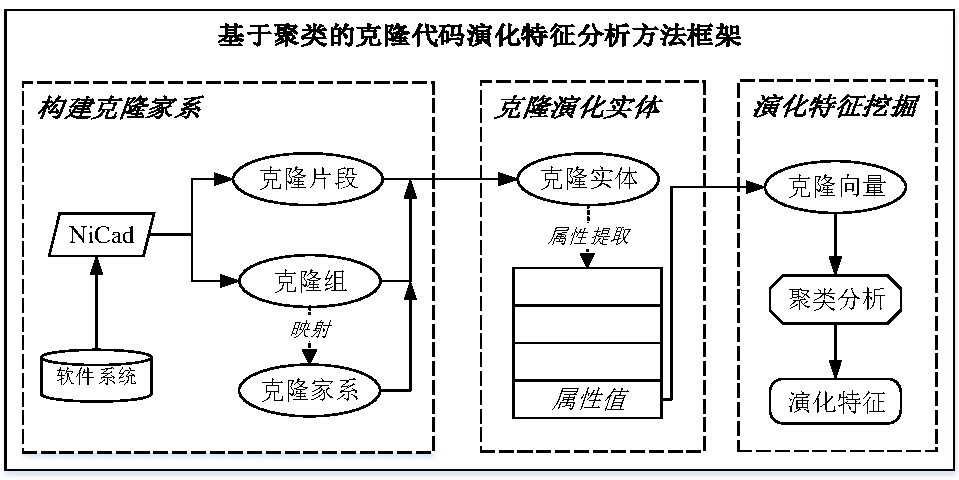
\includegraphics [width=0.75 \textwidth ]{framework2.pdf}
\bicaption [framework2]{}{基于聚类的克隆演化特征提取方法}
{Fig.$\!$}{The approach for clone characteristic analysis based on clustering}
\vspace{-1em}
\end{figure}

本章将克隆代码及其演化过程抽象成为“特征向量”,并借助机器学习中的聚类方法挖掘克隆代码的演化特征。在使用聚类分析的时候,由于克隆代码是具体的代码片段,无法直接对其聚类。因此,使用克隆聚类向量表示相应的克隆实体,而克隆聚类向量则是根据克隆实体相应的属性值生成,克隆实体的属性值用于表示克隆代码及其演化过程。本文从三种不同克隆实体表示克隆代码,即克隆片段、克隆组和克隆家系。克隆片段实体是微观角度,从克隆代码自身角度出发,将从克隆代码片段本身是否被修改的角度分析克隆代码的演化特征,所提取的度量值重点关注克隆代码是否被修改。克隆组实体是代码区域角度,从克隆组的角度分析克隆代码演化模式与演化时间的关系, 将揭示克隆组在随着软件演化时所表现出来的特征。克隆家系实体是宏观角度,描述了一个系统中所有克隆代码(即全部克隆家系)的演化过程以及演化特征。

本章所采用的聚类分析方法为 X-means\cite{pelleg2000x}聚类,其原因在于:克隆实体所应聚类的数量具有不确定性,难以确定具体的聚类数量。如果采用人为给定的方式给出聚类的数量,则可能会引入不客观因素,影响克隆代码演化特征的分析和提取。因此,本章采用X-means聚类方法,无需人为的指定聚类数量,X-means方法会自动地选择出最佳的聚类数量。

综上所述,本章基于软件演化和机器学习方法分析和挖掘克隆代码的演化特征,将重点分析讨论如下问题:

(1)如何结合软件演化过程,定义和模型化克隆代码的演化过程?

(2)如何从不同的角度描述和表示克隆代码及其演化过程,即如何从克隆片段、克隆组和克隆家系三个不同的角度分析克隆代码的演化情况?

(3)如何全面且客观地分析和挖掘克隆代码演化特征,并帮助开发人员理解和维护软件系统中的克隆代码?

\BiSection{克隆代码及演化过程的定义}
{Definitions for Code Clone and its Evolution}
\label{lab-evolution}

软件工程实践会产生大量的克隆代码,存在的克隆代码不仅使得系统变得更加臃肿,也使得系统越来越难以理解。为收集和检测系统中存在的克隆代码,在过去的20年中,提出了许多种克隆代码检测方法,并开发了大量的克隆检测工具,例如NiCad\cite{roy2008nicad}、CCFinder\cite{kamiya2002ccfinder}等(见本文绪论第~\ref{ref-detection}~节克隆代码检测)。

目前,大多数的克隆检测工具可以检测单版本系统中克隆代码,并向程序开发人员报告检测结果。克隆检测结果以克隆片段和克隆组的形式进行组织。克隆片段是具体克隆代码,克隆组是彼此相似的克隆片段的集合。克隆片段和克隆组可以描述如下:

\begin{definition}[克隆片段]
\label{defn-clonefragment}
克隆片段(Clone Fragment, CF)是彼此相似的代码片段,包括若干行连续的代码。给定两个代码片段$CF_1$和$CF_2$,如果$CF_1$和$CF_2$满足:
\begin{equation} 
  \begin{array}[t]{c}
    \mathit{TextSim}(CF_1, CF_2) > \mathit{sim\_th} \\
  \end{array}
\end{equation} 
则称代码片段$CF_1$和$CF_2$为克隆代码(CFs),其中$\mathit{TextSim}$为相似性度量,$\mathit{sim\_th}$为相似性阈值。
\end{definition}

本文使用NiCad\cite{roy2008nicad}检测系统中存在的克隆代码,因此$\mathit{TextSim}$采用NiCad中所的定义方法。在NiCad中,克隆代码相似性定义为$\mathit{TextSim}(CF_1, CF_2)$ = $1 - \mathit{UPI}(CF_1, CF_2)$。其中,UPI(Unique Percentage Items)表示两个代码片段之间不同的代码行数占总代码行的比例。假如给定两个代码片段$CF_1$和$CF_2$,其$\mathit{UPI}(CF_1,CF_2)=0.3$,表示两者的差异程度为30\%。同时,其相似度可根据UPI计算:$\mathit{SimText} (CF_1,CF_2) = 1- \mathit{UPI} = 0.7$,表示两者的相似度为70\%。本文将克隆代码的相似性阈值设置为0.7,当两个代码片段相似性大于0.7时,才被认定为是克隆代码。
与此同时,NiCad在检测克隆代码时会设定代码片段的长度范围为10 - 2500行,即代码行数在此范围内的代码片段会被检测为克隆代码。

\begin{definition}[克隆组]
\label {def-clonegroup}
克隆组 (Clone Group, CG)是彼此相似的克隆代码片段的集合,包含若干个彼此相似的克隆片段。假定$CF_i$和$CF_j$是一个克隆组$CG$中的任意两个克隆代码片段,则$CF_i$和$CF_j$满足
\begin{equation} 
  \begin{array}[t]{c}
    \mathit{TextSim}(CF_i, CF_j) > \mathit{sim\_th} \\
  \end{array}
\end{equation}
克隆组揭示了该克隆组内的克隆片段之间的克隆关系,即克隆组内的克隆片段互为克隆代码。
\end {definition}

如绪论中所述,克隆代码在系统中不是静止不变的,会随着软件系统的演化同时进行演化。克隆演化过程最早是2001年由Antoniol等人提出,使用时间序列描述克隆代码的演化模型\cite{antoniol2001modeling},但并未引起人们的重视。2005年,Kim提出了克隆家系模型用于描述克隆代码的演化过程,是迄今为止最好的用于描述克隆代码演化情况的模型\cite{kim2005empirical}。因此,本文也使用克隆家系模型描述克隆代码演化过程,所使用的克隆家系可以描述如下:

\begin{definition}[克隆家系]
\label{def-clonegenealogy}
克隆家系 (Clone Genealogy, CGE)是一个有向无环图,描述了一个克隆组($CG$)随着软件系统进行演化的过程。$CGE$图中的某一节点表示系统某一个版本($V_i$)中的该克隆组($CG_i$)。$CGE$图中的边表示该克隆组($CG$)在相邻的两个版本中$(V_{i-1},V_i )$的演化关系$(CG_{i-1},CG_{i})$,即该克隆组$CG$由上一版本$V_{i-1}$的$CG_{i-1}$演化至下一版本$V_{i}$中的$CG_{i}$。
\end{definition} 

在克隆代码的演化过程中,克隆代码可能会被开发人员修改而发生变化,因而也会导致两个相邻版本间的同一克隆组也会发生相应的变化。为了描述相邻版本之间的克隆组的变化情况,可以使用“克隆演化模式”进行描述。一个克隆组在两个相邻版本之间的克隆演化模式可以描述如下:

\begin{definition}[克隆演化模式]
\label{def-evolutionpattern}
克隆演化模式 (Clone Evolution Pattern, CEP)是某一克隆组($CG$)在相邻两个软件版本之间的演化情况。CEP描述该克隆组在相邻版本的变化情况,根据不同的演化情况具有7种不同的演化模式。假设该克隆组$CG$从系统版本$V_{i-1}$演化至$V_{i}$,其演化关系$(CG_{i-1},CG_{i})$可以定义如下:
%%%添加7种演化模式的具体的数学描述。
\begin{itemize}
\item 
静态模式 (Static Pattern):
静态模式表示在两个相邻版本的演化中该克隆组是静止的、未发生任何变化,即克隆组内的克隆片段数量和内容均未发生变化。克隆组$CG_{i-1}$和$CG_{i}$是相邻两个版本的同一克隆组,克隆组内的克隆片段是一一对应的,且对组内任意的一个克隆片段$CF_{i-1}$和$CF_{i}$,满足
\begin{equation} 
\begin{array}[t]{c}
  \mathit{TextSim}(CF_{i-1}, CF_i) = 1 \\
\end{array}
\end{equation}

\item 
相同模式(Same Pattern):
相同模式表示在两个相邻版本的演化中该克隆组内克隆片段数量无变化(但克隆片段本身可能发生变化)。克隆组$CG_{i-1}$和$CG_{i}$是相邻两个版本的同一克隆组,且克隆组$CG_{i-1}$和$CG_{i}$中的克隆片段数量分别为$N_{i-1}$和$N_{i}$,满足$N_{i-1} = N_{i}$。

\item 
增加模式(Add Pattern):
增加模式表示在两个相邻版本的演化中该克隆组内克隆片段增加。克隆组$CG_{i-1}$和$CG_{i}$是相邻两个版本的同一克隆组,克隆组$CG_{i-1}$和$CG_{i}$中的克隆片段数量分别为$N_{i-1}$和$N_{i}$,且克隆组映射的克隆片段的数量为$N$,增加模式满足$N < N_{i}$。

\item 
减少模式(Subtract Pattern):
减少模式表示在两个相邻版本的演化中该克隆组内的克隆片段减少。克隆组$CG_{i-1}$和$CG_{i}$是相邻两个版本的同一克隆组,克隆组$CG_{i-1}$和$CG_{i}$中的克隆片段数量分别为$N_{i-1}$和$N_{i}$,且克隆组映射的克隆片段的数量为$N$,满足$N_{i-1} > N$。

\item 
一致性变化模式(Consistent Change Pattern): 
一致性变化模式表示在两个相邻版本的演化中该克隆组内的克隆片段发生了一致地变化,并且发生变化的克隆片段仍然存在同一克隆组内。在从版本$V_{i-1}$演化到$V_{i}$的过程中,克隆组$CG_{i}$中的全部克隆片段发生了相同的变化(数量为$n$),即由$CF^{j}_{i-1}$变为$CF^{j}_i$($\forall j \in \{n\}$)。  如果对于接近于0的阈值$\tau$,克隆片段$CF^{j}_i$的变化满足以下条件,称此克隆组$CG_{i}$发生了一致性变化模式, 
\begin{equation}
\begin{split}
\begin{array}[t]{crl}
    \mathit{TextSim}(CF^{j}_{i-1}, CF^{j}_{i}) < 1, & \forall j \in \{n\} &(1)  \\
    {|~\mathit{TextSim}(CF^{p}_{i-1},CF^{p}_{i})-\mathit{TextSim}(CF^{q}_{i-1},CF^{q}_{i}) ~|~<~\tau},  & \forall {p,q} \in \{n\}& (2)
\end{array}
\end{split}
\end{equation}
  
\item 
不一致性变化模式(Inconsistent Change Pattern):
不一致性变化模式表示在两个相邻版本的演化中该克隆组内的克隆片段发生了不一致地变化,并且发生变化的克隆片段仍然存在同一克隆组内。$CG_{i}$的克隆片段发生了变化,但是不满足一致性变化模式的条件,称此克隆组$CG_{i}$发生了不一致性变化模式。

\item 
分裂模式(Split Pattern):分裂模式表示在两个连续版本的演化中克隆组内克隆片段发生了变化,并且导致在下一个版本中该克隆组分裂成为两个不同的克隆组。版本$V_i$中存在两个不同的克隆组$CG^p_i$和$CG^q_i$均是由上一版本$V_{i-1}$的克隆组$CG_{i-1}$演化而来,对克隆组$CG^p_i$和$CG^q_i$中任意的$CF^p_i$和$CF^q_i$满足:
\begin{equation}
\mathit{TextSim}(CF^{p}_{i}, CF^{q}_{i}) < \mathit{sim\_th}
\end{equation}
则称版本$V_i$中的克隆组$CG_i$发生了分裂模式。

\end{itemize}
\end{definition} 

为了更为形象的描述克隆家系及其演化模式,本文给出一个克隆家系的示意图,如图~\ref{genealogy1}~所示。从图中可以看出,克隆家系($CGE$)是克隆组($CG$)随着软件系统演化的一个有向无环图,图中的节点表示一个克隆组$CG$,图中边表示该克隆组在两个连续版本之间的演化关系$(CG_{i-1},CG_{i})$。同时,该克隆组的演化模式可以通过比较$CG_{i-1}$和$CG_{i}$中克隆代码片段获取。

\begin{figure}[htbp]
\centering
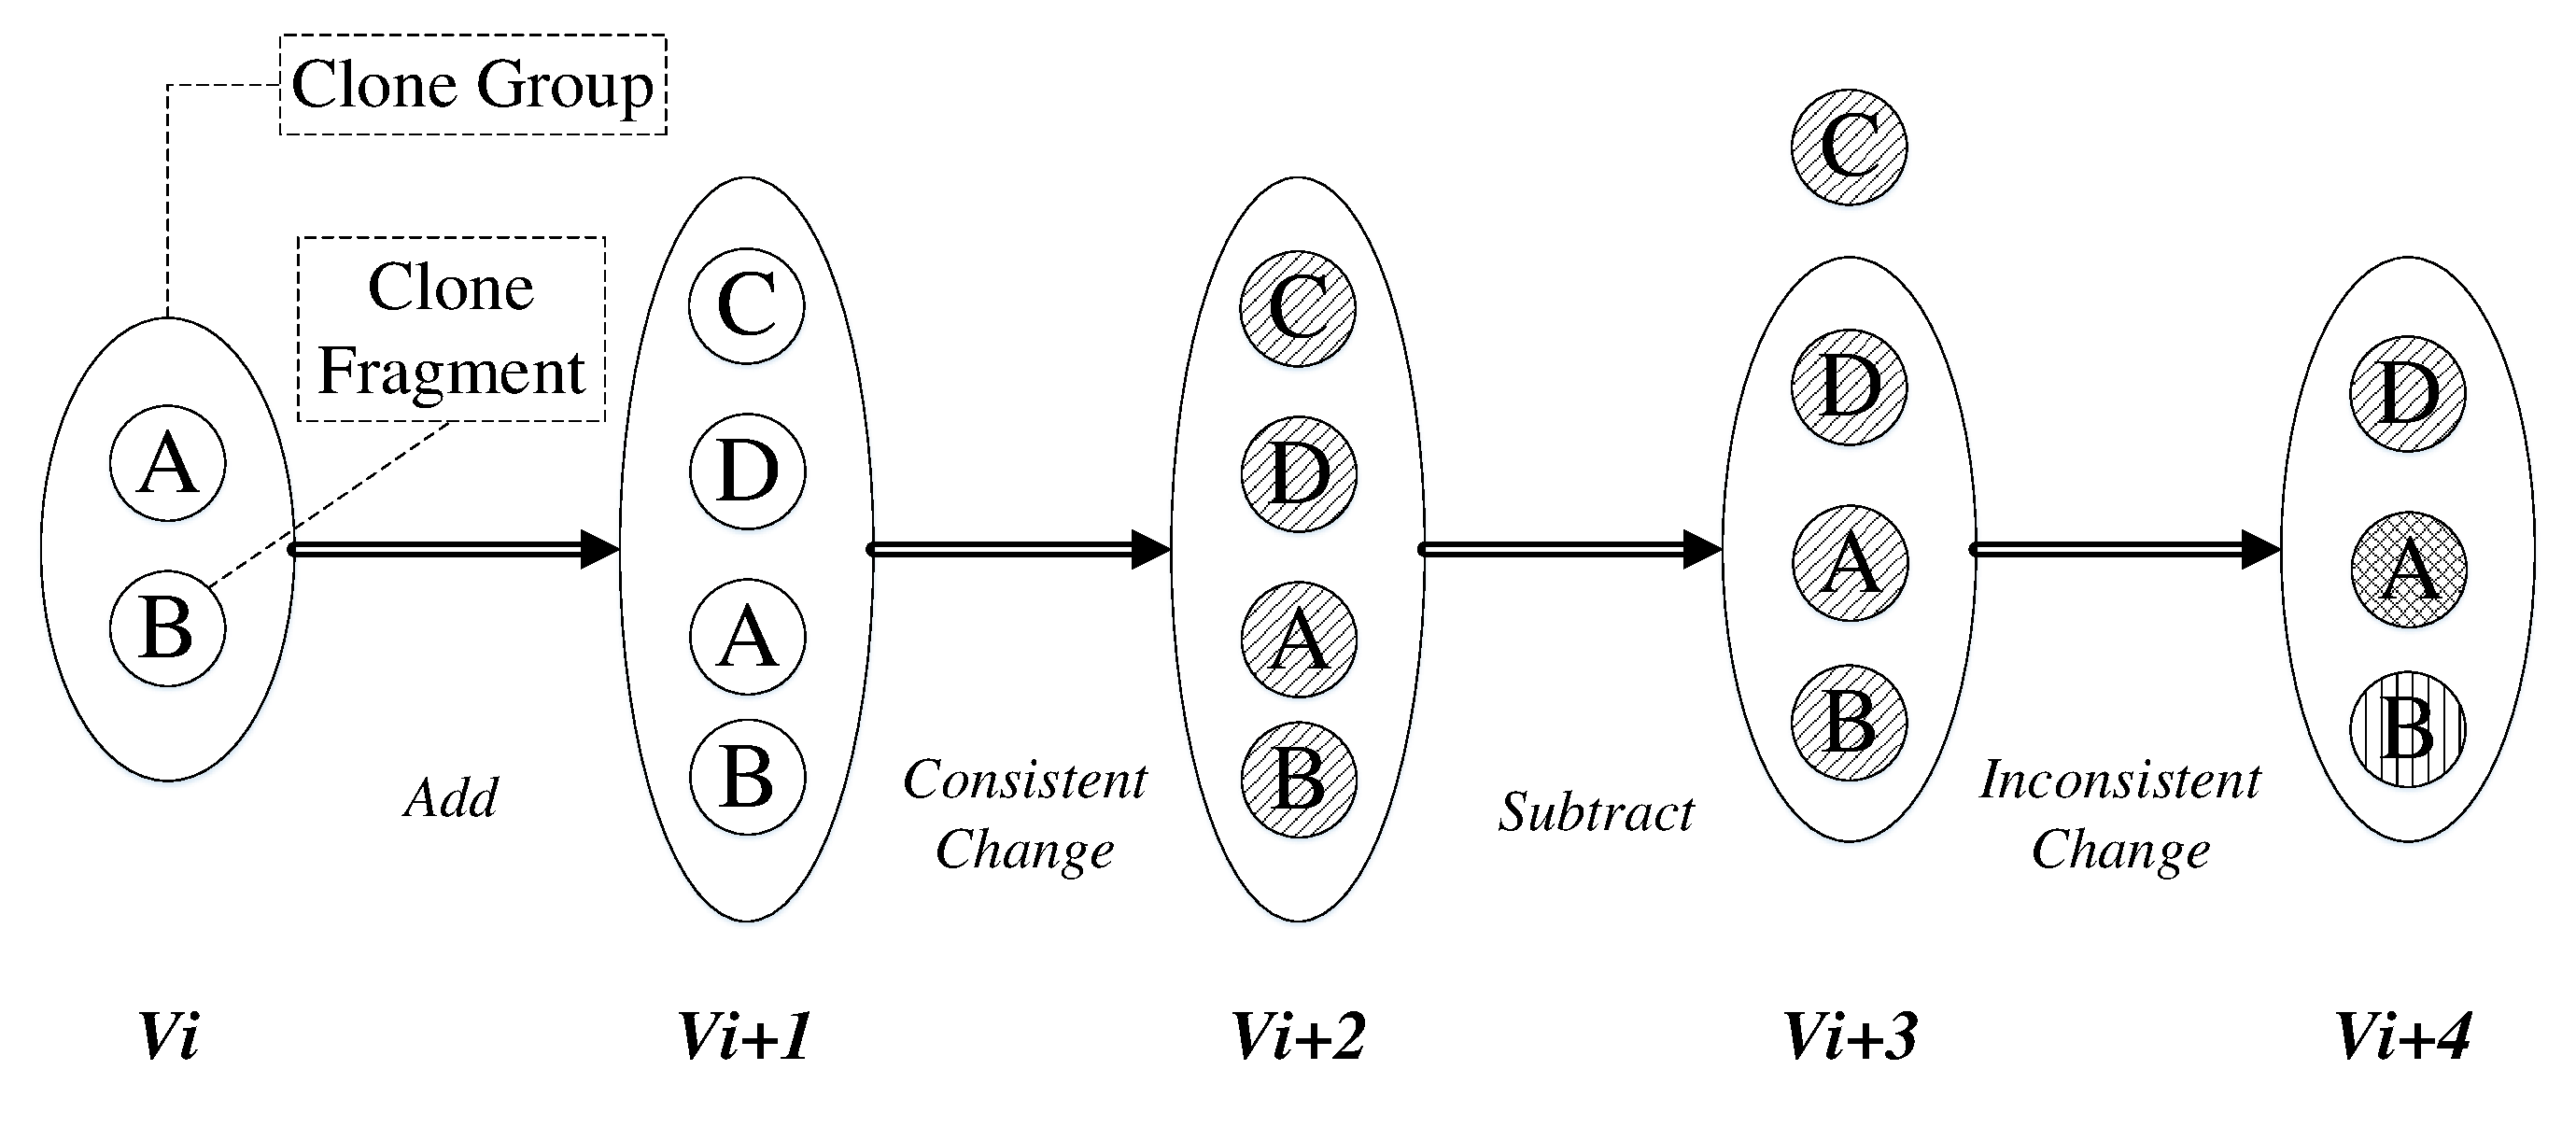
\includegraphics [width=0.75 \textwidth ]{genealogy1.pdf}
\bicaption [genealogy1]{}{克隆家系示意图\cite{kim2005empirical}}
{Fig.$\!$}{An example for clone genealogy\cite{kim2005empirical}}
\vspace{-1em}
\end{figure}

图~\ref{genealogy1}~也描述了一个克隆组$CG$在五个连续版本$(V_i, V_{i+4})$中的演化过程。从版本$V_i$到$V_{i+1}$,克隆组$CG$新增加了两个克隆片段,因此与之其关联的克隆模式是增加模式(Add Pattern)。从版本$V_{i+1}$到 $V_{i+2}$时,克隆组$CG$中全部的克隆代码片段发生了一致地变化,其克隆演化模式为一致性变化模式(Consistent Change Pattern)。从版本$V_{i+2}$到$V_{i+3}$时,克隆组$CG$中减少了一个克隆代码片段,其演化模式是减少模式(Subtract Pattern)。 从版本$V_{i+3}$到$V_{i+4}$时,克隆组中的克隆代码片段发生了不一致地变化,因此克隆演化模式为不一致性变化模式(Inconsistent Change Pattern)。

\BiSection{软件克隆家系的构建}
{Constructing Clone Genealogy for Software Repository}

在构建克隆家系阶段,使用克隆检测工具所检测的连续版本软件中的所有克隆代码,并通过映射相邻版本的克隆代码构建系统的克隆家系。首先,从开源库中下载连续版本软件的所有源代码。然后,使用克隆检测工具NiCad检测克隆代码。最后,通过映射克隆代码构建克隆家系并识别克隆演化模式。

\BiSubsection{克隆检测与CRD描述}
{Clone Detection and Representation with CRD}

本节使用克隆检测工具NiCad分别检测系统所有版本中的克隆代码,并使用克隆区域描述符(Clone Region Description,CRD)描述克隆代码的相关信息。

为了检测系统中的克隆代码,本文使用NiCad\cite{roy2008nicad}检测系统中的克隆代码。NiCad是基于文本的克隆检测工具,在工具中集成了程序转换、代码规范化和语法分析技术\cite{cordy2006txl,dean2003agile},能够以较高的准确度和召回率系统中的Type-1、Type-2和Type-3克隆代码\footnote{NiCad可从此网站获取:http://www.txl.ca/nicaddownload.html。}。NiCad可以从两个不同粒度检测系统中的克隆代码:函数粒度和块粒度。因为块粒度具有更为通用的检测效果(函数克隆也是是块克隆代码),本文使用块粒度检测系克隆代码。根据NiCad的默认配置,其将克隆代码之间的相似度阈值设置为70\%,将相似度高于此阈值的代码片段报告为克隆代码。

NiCad将检测到的克隆代码保存于XML文件中,并使用{“Filename + Start/End Line No.”}标记克隆克隆代码,并将彼此相似的克隆片段保存在同一克隆组内。由于NiCad仅仅使用代码行表示克隆代码,不仅无法描述克隆代码的语法和语义信息,也不利于映射不同版本之间的克隆代码。因此,为映射相邻版本之间的克隆代码,本文使用克隆区域描述符表示克隆代码,并在此基础上实现克隆代码的映射和克隆家系的构建。

克隆区域描述符最早由Duala-Ekoko等人提出,不仅可以反映出克隆代码本身的信息,还可以用于跟踪演化过程中的克隆代码\cite{duala2010clone}。CRD能够充分地反映出克隆代码本身的信息,还能够反映克隆代码区域的特征,CRD的描述如图~\ref{crd}~所示。

\begin{figure}[h]
\centering
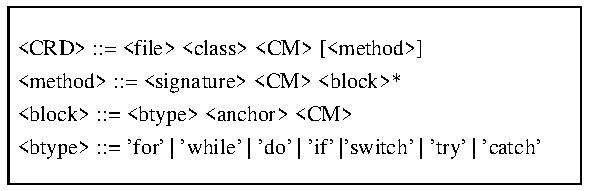
\includegraphics [width=0.6 \textwidth ]{CRD.pdf}
\bicaption [crd]{}{克隆区域描述符示意}
{Fig.$\!$}{The definition of clone region description}
\vspace{-1em}
\end{figure}

CRD克服了使用文件行描述克隆代码的局限,不依赖于克隆区域的具体位置,同时也独立于具体文本。使用CRD可以映射相邻版本之间的克隆代码,慈蒙等人改进了克隆区域描述符,并提出了基于克隆区域描述符的克隆群映射算法\cite{ci2013new}。同时,为了映射两个相邻版本中的克隆代码和克隆组,新添加相对位置覆盖率和文本相似度两个额外的表示单元。使用相对位置覆盖率可以帮助定位源代码中的克隆片段,并计算版本$V_i$和版本$V_{i+1}$中克隆片段位置之间的重叠率。文本相似度可以用于比较映射的代码片段的相似性度。

\BiSubsection{克隆家系构建与克隆模式识别}
{Building Clone Genealogy and Identifying Clone Evolutionary Pattern}

为了映射连续版本的克隆代码,使用基于克隆区域描述符的映射算法,生成所有相邻版本的映射结果,并根据映射结果构建克隆家系和识别克隆演化模式。

构建克隆家系的关键步骤在于映射所有相邻版本间的克隆片段。而相邻版本间的克隆群映射关系,则可以根据克隆群内的克隆片段的映射关系进行确定。所采用的映射算法称为基于CRD的克隆代码映射算法\cite{ci2013new}。假设给定一个软件系统的两个相邻版本{$V_i$}和{$V_ {i + 1}$},并分别给出两个版本之间的克隆代码,并使用CRD描述所检测到的克隆代码。为了映射两个版本间的克隆代码,将{ $V_i$}中的每个克隆片段与下一版本{$ V_{i+1}$}中的每个克隆片段进行比较,寻找与之映射的克隆片段,并生成克隆片段的映射结果。于此同时,根据克隆片段的映射结果,也可以实现相邻版本中所有克隆组的映射。更进一步,将所有相邻版本之间的克隆代码进行映射,可以通过遍历映射结果生成系统中的所有的克隆家系。

与此同时,克隆演化模式可以用于描述克隆组在演化过程中的变化情况,对于揭示克隆演化特征具有重要的意义。克隆演化模式识别,可以通过对比映射的两个相邻版本之间的克隆组进行。假设克隆组$CG$是存在于相邻的两个软件版本{$(V_i,V_{i+1})$}中,且克隆组$CG$的映射关系可以使用{$(CG_i, CG_{i+1})$}描述,其中{$CG_i$}表示前一版本中的克隆组,{$CG_{i+1}$}表示后一版本中的克隆组。通过观察从{$CG_i$}到{$CG_{i+1}$}的克隆组变化情况,便可以识别该克隆组{$CG_{i+1}$}的克隆演化模式。

构建克隆家系的算法如~\ref{alg-building}~所示。算法中第1 - 3行是为所检测到的每一个克隆代码生成CRD描述,并将结果保存。第4 - 6行是使用基于CRD克隆群映射算法映射相邻版本的克隆代码,同样将结果保存起来。第7 - 10行根据克隆演化模式定义,识别所有映射的相邻版本的克隆组的克隆演化模式。第11行通过遍历映射文件生成系统中全部的克隆家系。假设一个版本中有$m$个克隆代码,生成CRD所需时间为$O(m)$。软件系统的$n$版本需时间为$O(m*n)$。映射克隆相邻版本的克隆代码以及识别演化模式的时间复杂度同样为$O(m*n)$。所以该算法的复杂度为$O(m*n)$。

\vspace{1em}
\begin{minipage}{0.8\textwidth}
\centering
\begin{algorithm}[H]
\AlgoBiCaption{克隆家系构建与演化模式识别算法}
{Algorithm for building CGEs and identifying CEPs}
\label{alg-building}
\KwIn{All source code and code clones from $N$ versions}
\KwOut{All clone genealogies $CGEs$}
%\Comment{生成CRD描述克隆代码片段\;}
\For{$i$=1 to $N$}
{ 
 Generating CRD for represent each $CF_i$ in version $i$\;
 Saving all results in {result\_i} files\;
}
%\Comment{映射相邻版本的$CFs$和$CGs$}
\For{$i$=1 to $N-1$}
{ 
 Mapping all the $CFs$ and $CGs$ between adjacent versions {$i$} and {$i+1$}\;
 Saving all mapping results in {mapping\_i} files\;
}
%\Comment{识别演化模式}
\For{$i$=1 to $N-1$}
{
	\For{each mapping $CGs$ in version $i$ and $i+1$}
	{
	Identify all clone patterns {CEPs} in thus two versions according to Definition~\ref{def-evolutionpattern}~\;
	Saving all mapping results in {mapping\_i} files\;
	}
}
Generating all clone genealogies $CGEs$ through traversing all mapping files\;
\Return {$CGEs$\;}
\end{algorithm}
\end{minipage}
\vspace{1em}

\BiSection{克隆演化实体的特征描述}
{The Attributes for Three Clone Evolution Entities}

为挖掘克隆代码的演化特征,本节从三个不同的角度表示克隆代码及其演化情况,即克隆片段、克隆组和克隆家系,并将之称为克隆演化实体(简称为克隆实体)。对克隆片段实体,重点关注克隆代码片段的变化情况。对克隆组实体,重点关注克隆组的克隆演化模式分布情况。对于克隆家系实体,重点关注克隆组在整个演化过程中的演化情况。

\BiSubsection{克隆片段实体的特征}
{The Attributes for Clone Fragment Entity}

克隆代码片段是最小的克隆演化实体单元。克隆片段实体描述了克隆代码本身的一些特征。在克隆片段的生命期间,克隆片段可能被软件人员开发人员修改(特别是在软件维护期间)。因此,克隆片段在演化过程中可能会发生变化,甚至在其演化过程中可能发生不止一次的变化。

因此,对于克隆片段实体,将重点考虑其变化情况。某一版本$V_i$的克隆片段实体,将提取其两个属性特征表示克隆片段实体,即历史变化次数(截止到版本$V_i$)和是否发生了变化(从上一版本$V_{i-1}$演化到此版本$V_i$时)。同时,也会提取克隆片段实体的寿命作为另一个重要的属性特征。因此,对某一克隆片段实体$CF$,其所在的软件版本为$V_i$,该克隆片段实体$CF_i$的属性特征可描述如下:

\begin{itemize}
\item
克隆片段寿命(Clone Fragment Life):
截止到当前版本$V_ i $,克隆片段$CF_i$所经历的所有的版本数量称之为克隆片段寿命。假定起始版本为$V_s$,克隆寿命为$i - s$。
%\item {Clone Life}: number of versions which the clone fragment exists in software so far (until version i).
\item
是否发生变化(Ischanged):
从上一版本$V_{i-1} $演化到当前版本$V_i $时,克隆片段$CF_i$是否发生了变化。如果$\mathit{TextSim}(CF_{i-1}, CF_{i}) < 1$,则取值为$1$,否则取值为$0$。
%\item {Ischanged}:	equals 1 if the Clone fragment in version i is changed from the last version (version i-1); 0 otherwise.
\item
变化次数(Change Times):
截止到当前版本$V_ i $,克隆片段$CF_i$在其演化过程中所发生的变化次数。假定克隆片段的初始版本为$V_s$,变化次数为:$\sum_{j=s}^i{ischanged_j}$
%\item {Change Times}:	number of times the clone fragment changed so far (up till version i) in the evolution.  
\end{itemize}

\BiSubsection{克隆组实体的特征}
{The Attributes for Clone Group Entity}

克隆片段实体仅从单个克隆代码的角度描述了克隆演化中的被修改的情况。而克隆组实体可以提供一些克隆代码的区域性特征。克隆代码演化模式描述了相邻版本之间的克隆组的演化情况,因此,可以使用克隆组当前的演化模式描述克隆组实体在相邻两个版本之间的变化情况。

对于某一个演化中的克隆组实体,从上一版本演化至当前版本时,其克隆演化模式可以作为克隆组实体的属性特征。同时,其存在于软件中的时间(克隆组寿命),同样也是一个重要的属性特征。克隆组寿命不但揭示了其在系统中存在的时间长短,也可能与克隆演化模式息息相关。因此,本节将克隆组的寿命和当前的演化模式视为克隆组实体的属性特征。对某一克隆组$CG$,其所在的软件文版本为$V_i $ ,该克隆组实体{$CG_i$}的属性特征可以描述如下:

\begin{itemize}
\item
克隆组寿命(Clone Group Life):
截止到当前版本$V_ i $,克隆组$CG_i$所经历的所有的版本数量称之为克隆组寿命。
%\item {Group Life}: number of versions which clone group exists in software till version $i$.
\item
当前静态模式(Current Static Pattern):
克隆组$CG_i$从上一版本$V_{i-1} $演化到$V_i $时,是否发生了静态模式(Static Pattern),若发生取值为1,反之为0。
%\item {Static}:	all clone fragments in group are static from last version.
\item
当前相同模式(Current Same Pattern):
克隆组$CG_i$从上一版本$V_{i-1} $演化到$V_i $时,是否发生了相同模式(Same Pattern),若发生取值为1,反之为0。
%\item {Same}:	clone group undergoes a ``same'' pattern change from  last version.
\item
当前增加模式(Current Add Pattern):
克隆组$CG_i$从上一版本$V_{i-1} $演化到$V_i $时,是否发生了增加模式(Add Pattern),若发生取值为1,反之为0。
%\item {Add}: clone group undergoes an ``add'' pattern change from last version.
\item
当前减少模式(Current Subtract Pattern):
克隆组$CG_i$从上一版本$V_{i-1} $演化到$V_i $时,是否发生了减少模式(Subtract Pattern),若发生取值为1,反之为0。
%\item {Subtract}: clone group undergoes a ``subtract'' pattern change from last version.
\item
当前一致性变化模式(Current Consistent Change Pattern):
克隆组$CG_i$从上一版本$V_{i-1} $演化到$V_i $时,是否发生了一致性变化模式(Consistent Change Pattern),若发生取值为1,反之为0。
%\item {Consistent Change}: clone group undergoes a ``consistent change'' pattern from last version.
\item
当前不一致变化模式(Current Inconsistent Change Pattern):
克隆组$CG_i$从上一版本$V_{i-1} $演化到$V_ i $时,是否发生了不一致变化模式(Inconsistent Change Pattern),若发生取值为1,反之为0。
%\item {Inconsistent Change}: clone group undergoes an ``inconsistent change'' pattern from last version.
\item
当前分裂模式(Current Split Pattern):
克隆组$CG_i$从上一版本$V_{i-1} $演化到$V_i $时,是否发生了分裂模式(Split Pattern),若发生取值为1,反之为0。
%\item {Split}: clone group undergoes a ``split'' pattern change from last version.
\end{itemize}

\BiSubsection{克隆家系实体的特征}
{The Attributes for Clone Genealogy Entity }

克隆家系实体是克隆代码演化的全局视角,提供了某一克隆组在其整个演化过程中的演化情况,可以帮助捕获软件系统中全部克隆代码的演化情况。如前文所述,一个克隆组在所有的版本中的全部演化过程是一个克隆家系。因此,在其整个演化过程中,其所经历的所有的演化模式数量,可以描述克隆家系实体的在其整个演化过程中的整个变化历史演化过程。同时,对于一个克隆家系,克隆寿命是克隆家系的另一个重要的指标,描述了克隆代码在系统中存在的时间。

因此,克隆家系实体的寿命和克隆演化模式数量可以作为克隆家系实体的属性特征。对于某一克隆家系实体{$CGE$},该克隆家系实体{$CGE$}的属性特征可以描述如下:

\begin{itemize}
\item
克隆家系寿命(Clone Genealogy  Life):
克隆家系{$CGE$}在其整个演化过程中所经历的软件版本的数量。
%\item Genealogy  Life: number of versions which clone genealogy exists in software.
\item
静态模式数量(Static Pattern Number):
克隆家系{$CGE$}在其整个演化过程中所经历的静态模式的数量。
%\item Static Number: number of ``static'' pattern which all clone groups belonging to this genealogy have experienced in its life.
\item
相同模式数量(Same Pattern Number):
克隆家系{$CGE$}在其整个演化过程中所经历的相同模式的数量。
%\item Same Number: number of ``same'' pattern which all clone groups belonging to this genealogy have experienced in its life.
\item
增加模式数量(Add Pattern Number):
克隆家系{$CGE$}在其整个演化过程中所经历的增加模式的数量。
%\item Add Number: number of ``add'' pattern which all clone groups belonging to this genealogy have experienced  in its life.
\item
减少模式数量(Subtract Pattern Number):
克隆家系{$CGE$}在其整个演化过程中所经历的减少模式的数量。
%\item Subtract Number: number of ``subtract'' pattern which all clone groups belonging to this genealogy have experienced in its life.
\item
一致性变化模式数量(Consistent Change Pattern Number):
克隆家系{$CGE$}在其整个演化过程中所经历的一致性变化模式的数量。
%\item Consistent Number: number of ``consistent pattern'' which all clone groups belonging to this genealogy have experienced in its life.
\item
不一致变化模式数量(Inconsistent Change Pattern Number):
克隆家系{$CGE$}在其整个演化过程中所经历的不一致变化模式的数量。
%\item Inconsistent Number: number of ``inconsistent pattern'' which all clone groups belonging to this clone genealogy have experienced in its life.
\item
分裂模式数量(Split Pattern Number):
克隆家系{$CGE$}在其整个演化过程中所经历的分裂模式的数量。
%\item Split Number: number of ``split'' pattern which all clone groups belonging to this genealogy have experienced in its life.
\end{itemize}

\BiSection{克隆演化特征挖掘}
{Mining Clone Evolutionary Characteristics}

为分析克隆代码及其演化过程,使用不同的属性特征分别描述克隆片段实体、克隆组实体和克隆家系实体,并采用X-means\cite{pelleg2000x}聚类方法挖掘和分析克隆代码演化特征。克隆实体所应聚类的数量具有不确定性,难以确定具体的聚类数量。如果采用人为给定的方式给出聚类的数量,则可能会引入不客观因素,影响克隆代码演化特征的分析和提取。X-means聚类方法是K-means聚类方法的改进方法,在使用其聚类时无需指定聚类数量,方法会自动地选择出最佳的聚类数量。本节将使用WEKA( “Waikato Environment for Knowledge Analysis” \cite{hall2009weka})中提供的X-means聚类方法来分析克隆演化实体,将从克隆片段、克隆组和克隆家系三个不同的角度分别对克隆代码及其演化过程进行聚类分析。

\BiSubsection{克隆实体聚类向量的生成}
{Generating the Clustering Vectors for Clone Entities}

使用X-means聚类克隆代码实体,需要生成与之对应的克隆聚类向量空间。这一过程可以划分为两个子步骤:首先,为每一个克隆代码实体成一个“克隆聚类向量”,该向量包含某个克隆实体的所有属性值。然后,使用克隆实体全部的“克隆聚类向量”生成所有克隆实体的“聚类空间”,包含克隆片段、克隆组和克隆家系三个聚类空间。

(1)为每一个克隆代码实体生成克隆聚类向量

对于每个克隆片段、克隆组和克隆家系实体,其聚类向量是一个$m$维向量:{$Vector$ = {($v_1$,$v_2$,$...$,$v_m$)}},其中$v_i$表示该克隆实体的一个特定属性值。以某一克隆组{$CG_i$}为例,为该克隆组实体{$CG_i$}生成一个8维向量{$Vector(CG_i)$ = ($v_1$,$v_2$,$...$,$v_8$)},其中$v_i$(对于所有$i$ , $i \leq $ 8)是此克隆组{$CG_i$}所对应的属性值。$Vector(CG_i)$即为克隆组实体{$CG_i$}的克隆聚类向量。
 
(2)生成所有克隆代码实体的聚类向量空间

为了聚类所有的克隆实体,还行生成系统的全部克隆聚类向量空间。假设由所有克隆实体的聚类向量生成的聚类向量空间为$X$,则$X$可由{$X$={($x_1$,$x_2$,$...$,$x_n$)}}表示,其中$n$是全部克隆实体的数量。本章从克隆片段实体、克隆组实体和克隆家系实体三个不同角度,聚类分析克隆代码及其演化过程。因此,本节也将生成三个不同的克隆向量空间:$X_{CF}$、$X_{CG}$和$X_{CGE}$,其中$X_{CF}$表示所有的克隆片段实体的聚类空间,$X_{CG}$表示所有克隆组实体的聚类空间,$X_{CGE}$表示所有克隆家系实体的聚类空间。

\BiSubsection{基于X-means的克隆实体聚类}
{Clustering All Clone Entities with X-means Method}

使用X-means方法聚类所有的克隆实体向量($X_{CF}$、$X_{CG}$和$X_{CGE}$),并根据聚类结果分析和提取克隆代码演化特征。

本章将使用WEKA中实现的聚类方法,实现对克隆实体的聚类。WEKA是由新西兰怀卡托大学开发的机器学习工具,WEKA中实现了许多方法来分析数据,例如聚类,分类,关联规则等\footnote{WEKA网站为:http://www.cs.waikato.ac.nz/ml/weka/。}。 由于上一节所生成克隆代码的向量空间为$X_{CF}$、$X_{CG}$和$X_{CGE}$,分别代表了系统中全部的克隆片段实体、克隆组实体和克隆家系实体。因此,也将使用X-means方法聚类这三个不同的向量空间,并分析得到克隆代码的演化特征。

本文使用的聚类方法是X-means聚类\cite{pelleg2000x}, X-means聚类是K-means聚类\cite{arthur2007k}的改进方法。K-means方法可以将向量空间$X$聚类为事前指定的$K$个Cluster中,并将彼此相似的向量分配到同一个Cluster中。但是,K-means聚类方法必须指定所需要聚类的Cluster的数量。然而,对于克隆代码实体的聚类而言,由于缺少必要的基本信息,难以确定所需的Cluster的数目。同时,人为的指定聚类的个数也会引入主观的因素。因此,本章选择使用X-means聚类方法。X-means聚类改进了K-means聚类方法,聚类时并不需要指定具体的Cluster数量。X-means聚类会自动的搜索最佳的Cluster数量,因此更为适合于克隆代码演化特征的聚类分析。

X-means聚类是一种高效的聚类算法,可以通过自动搜索并确定聚类数量\cite{pelleg2000x}。给定一个克隆实体的克隆向量空间$X$ = {($x_1$,$x_2$,$...$,$x_n$)},其中每个$x_i$是$d$维克隆演化实体的向量)。X-means聚类将向量空间$X$ 中的$n$个向量划分为$k$个Clusters,即 $C$ = {($c_1$,$c_2$,$...$,$c_k$)},$c_i$表示一个Cluster。$c_i$则表示了彼此比较相似的克隆代码实体,根据聚类结果可以进行克隆演化特征的挖掘。使用X-means聚类仅需要指定$K$的范围即可,聚类算法会自动的搜索最佳的Cluster数量$K$。聚类分析的结果见后文的实验分析部分。

最后,根据聚类分析的结果,可以进行挖掘和分析克隆代码的演化特征。
%%%描述X-means聚类
%过程如下:算法从给定的$K$范围的最低值开始,并继续增加此值,直到范围的上限。在此过程中,X-means聚类使用模型选择标准计算每个$K$的分数。它选择$K$的最高分数输出。对于每个$K$,x-means聚类使用迭代细化技术。首先,它将每个向量分配给其平均值产生集群内最小平方和(WCSS)的集群。第二,它计算新的均值为新聚类中的向量的质心。当分配不再改变时,算法收敛。它使用后验概率用贝叶斯信息准则对这$j$进行评分。

\vspace{1em}
\begin{minipage}{0.9\textwidth}
\centering
\begin{algorithm}[H]
\AlgoBiCaption{克隆演化特征聚类算法} {Algorithm of clustering for clone characteristics}
\label{alg-characteristic}
\KwIn{All clone genealogies $CGEs$ and all source code}
\KwOut{All clusters for clone fragments, groups, and genealogies}
Collecting all entities of clone genealogy with number {$N\_cge$}\;
Collecting all entities of clone group with number{$N\_cg$}\;
Collecting all entities of clone fragment with number {$N\_cf$}\; 
Initializing the clustering space of  $X_{CF}$, $X_{CG}$, and $X_{CGE}$\;
\For {$i$=1 to $N\_cge$}
{
 Generating the vector {$V\_i$} for {CGE\_i}\;
 Appending the vector {$V\_i$} to $X_{CGE}$\;
 }
\For {$i$=1 to $N\_cg$}
{ 
 Generating the vector for {CG\_i}\;
 Appending the vector {$V\_i$} to $X_{CG}$\;
}
\For {$i$=1 to $N\_cf$}
{ 
 Generating the vector {$V\_i$} for {CF\_i}\;
 Appending the vector {$V\_i$} to $X_{CF}$\;
}
Calling WEKA to clustering $X_{CF}$, $X_{CG}$ and  $X_{CGE}$ with X-means method\;
Mining clone evolutionary characteristic with the clusters of $X_{CF}$, $X_{CG}$ and  $X_{CGE}$\;
\Return {All clusters for clone fragment, group, and genealogy\;}
\end{algorithm}
\end{minipage}
\vspace{1em}

克隆演化特征的聚类算法如~\ref{alg-characteristic}~所示。算法的第1 - 3行分别收集系统中全部的克隆实体,分别为克隆家系实体、克隆组实体和克隆片段实体。第4行初始化三种克隆实例的聚类向量空间。第5 - 7行、8 - 10行、11 - 13行分别使用上文描述的属性生成克隆实体的聚类向量,并将其添加到聚类向量空间中。最后,第14行调用WEKA聚类克隆实体。收集不同克隆实体的算法复杂度为$O(m)$。算法的主要时间消耗在了生成克隆实例的向量空间上,其时间复杂度为$O(n*m)$,$n$为系统的版本数量。所以,该算法的时间复杂度为$O(n*m)$。

\BiSection{实验结果与分析}
{The Experimental Results and Analysis}
\label{ref-characteristics}

\BiSubsection{实验设置}
{Experimental Methodology}

本章选择了两个Java开源软件作为实验系统:分别为ArgoUML和 jEdit。ArgoUML是一个领先的开源UML建模工具,包括对所有标准UML 1.4图的支持。jEdit是程序员开发所使用的编辑器,其特点是具有易于使用的接口,类似于许多流行的文本编辑器。

表~\ref{statisticsofcluster}描述了这两个实验系统的基本信息。从表中第2 - 4列给出了系统的版本信息,ArgoUML经历了$14 $个版本的演化(起始和结束版本分别为$0.20.0$和$0.34.0$), jEdit经历了$22$个版本的演化(起始和结束版本分别为$3.0.0$和$5.0.0$)。表中第5 - 7列则给出了实验系统的克隆实体的数量(即克隆聚类空间大小)。其中,“Clone Fragment”列出了所聚类的克隆片段的数量,“Clone Group”和“Clone Genealogy”则分别是所聚类的克隆组和克隆家系数量。

\begin{table}[htbp]
\bicaption [statisticsofcluster]{}{两个开源软件实验系统信息}
{Table$\!$}{The information for two open sources experimental projects }
\vspace{0.5em}
\centering 
\wuhao
\begin{tabular}{ccccccc}
\toprule[1.5pt ]
\multirow{2}{*}{实验系统}&\multirow{2}{*}{版本数}&Start&End&Clone&Clone&Clone\\ 
&&Version&Version&Fragment&Group&Genealogy\\
\midrule[1pt]
ArgoUML&14&0.20.0&0.34.0&25422&7012&1036\\ 
jEdit&22&3.0.0&5.0.0&6636&2256	&237\\ 
\bottomrule[1.5pt]
\end{tabular}
\end{table}

本章从三个不同的视角挖掘和分析克隆代码的演化特征,即克隆片段、克隆组和克隆家系。因此,克隆演化特征的实验也可以划分成为三个部分:
\begin{itemize}
\item 克隆片段演化特征分析实验:
在克隆片段实验中,聚类克隆片段实体的向量空间,将分析克隆片段在演化过程中的变化情况,挖掘克隆片段变化的演化特征。 
\item 克隆组演化特征分析实验:
在克隆组实验中,聚类克隆组实体的向量空间,将分析克隆组在演化过程中的克隆演化模式情况,并挖掘克隆组实体的一致性和不一致变化模式。
\item 克隆家系演化特征分析实验:
在克隆家系的实验中,聚类克隆家系实体的向量空间,从全局的角度分析了系统中全部克隆代码的演化规律,并挖掘在整个演化过程中克隆代码的稳定性以及一致性变化的演化特征。
\end{itemize}

在每个实验中,本章将克隆代码演化特征的挖掘分成两个子任务。第一个子任务,对获得的所有克隆实体进行统计分析,并且根据统计分析结果获取克隆代码的演化特征。第二个子任务,使用WEKA对克隆实体进行聚类分析,根据聚类结果挖掘和分析克隆代码的演化特征。因此,均使用两种方法分析和挖掘克隆代码的演化特征:统计分析方法和聚类分析方法。第一种统计分析每种克隆实体的属性值分布情况,帮助发现一些最基本的分布特征。第二种是聚类分析方法,使用X-means分别聚类每一种克隆实体,并根据聚类结果深入挖掘在演化中克隆代码的演化特征。

\BiSubsection{克隆片段演化特征分析实验}
{Experiment for Clone Fragment Evolutionary Characteristics}

克隆片段是软件中存在的真实的代码片段, 在其生命周期内,克隆片段可能会被开发人员修改。本章考虑克隆片段实体的三个属性特征,分别是克隆寿命(Clone Life)、是否发生变化(Ischanged)和历史变化次数(Change Times),将帮助挖掘克隆片段在其演化过程中的真实变化情况。

\BiSubsubsection{克隆片段统计分析实验}
{Clone Fragment Experiment of Statistics}

对克隆片段的“历史变化次数”进行统计分析,分析结果如表~\ref{cfstaargouml}~(ArgoUML系统)和表~\ref{cfstajedit}~(jEdit系统)所示。表中详细给出了克隆代码片段的变化情况,其中数字“$0$”表示未发生变化,数字“$N$”表示了截止到当前版本克隆片段发生了{\emph N\/}次变化。同时,表中第三行给出了没有发生变化和发生变化的克隆片段的数量和比例。

\begin{table}[htbp]
\bicaption[cfstaargouml]{}{ArgoUML中克隆片段的变化情况统计}
{Table$\!$}{The statistic of clone fragment change for ArgoUML}
\vspace{0.5em}
\centering
\wuhao
\begin{tabular}{ccccc}
\toprule[1.5pt]
Change Times&0&1&2&3\\ 
\midrule[1pt]
数量&24327&982&109&4\\ 
%\cline{3-5}
总数&24327(95.69\%)&\multicolumn{3}{c}{1095(4.31\%)} \\
\bottomrule[1.5pt]
\end{tabular}
\end{table}

\begin{table}[htbp]
\bicaption[cfstajedit]{}{jEdit中克隆片段的变化情况统计}
{Table$\!$}{The statistic of clone fragment change for jEdit}
\vspace{0.5em}
\centering
\wuhao
\begin{tabular}{ccccccccc}
\toprule[1.5pt]
Change Times &0&1&2&3&4&5&6&7\\ 
\midrule[1pt]
数量&5885&533&135&47&14&10&11&1\\ 
%\cline{3-9}
总数&5885(88.68\%)&\multicolumn{7}{c}{751(11.32\%)}   \\ 
\bottomrule[1.5pt]
\end{tabular}
\end{table}

从表~\ref{cfstaargouml}~和表~\ref{cfstajedit}~中可以看出,大多数克隆片段在演化过程中并不会发生变化。未发生变化的克隆片段数量在ArgoUML中为$24327$个(其比例为95.69\%),在jEdit中为$5885$个(比例为88.68\%)。同时,只有仅仅一小部分克隆片段在演化过程中发生了变化,ArgoUML为$1095$个(比例为4.31\%),jEdit为$751$个(比例为11.32\%)。值得注意的是,在发生变化的克隆片段中,仅有极少数的克隆片段被改变了不止一次,其数量随着改变次数的增大而减少。

 因此,克隆片段在其生命期间是十分稳定的,大多数克隆片段从未发生过变化(比例分别为95.69\%和88.68\%)。但是,依然存在一定数量的克隆代码片段发生了变化。在发生变化的克隆片段中,克隆变化不会频繁地发生,仅有极少量的克隆代码会频繁的发生变化(发生多次变化)。
\BiSubsubsection{克隆片段聚类分析实验}
{Clone Fragment Experiment of Clustering}

使用X-means方法对克隆片段进行聚类分析,实验结果如表~\ref{cfcluargouml}~和~\ref{cfclujedit}~所示。从表中可以看出,X-means聚类将ArgoUML和jEdit的克隆代码片段实体分成4个Cluster:Cluster0 - Cluster3。根据其聚类结果分别统计了四个Cluster中克隆片段实体的属性特征信息,即克隆寿命(Clone Life)、是否发生变化(Ischanged)和变化次数(Change Time)。对上述每一种属性特征,表中使用平均值(Mean)、标准差(Standard Deviation,SD)和中位数(Median)来描述每一个Cluster中的属性的分布情况。

\begin{table}[htbp]
\bicaption[cfcluargouml]{}{ArgoUML中克隆片段的聚类结果}
{Table$\!$}{Clustering results of clone fragment for ArgoUML}
\vspace{0.5em}
\centering
\footnotesize
%\wuhao
\begin{tabular}{ccccccccccc}
\toprule[1.5pt]
\multirow{2}{*}{Cluster}&{数量}&\multicolumn{3}{c}{Clone Life}&\multicolumn{3}{c}{Ischanged}&\multicolumn{3}{c}{Change Times} \\
\cline{3-11}
&(比例)&{Mean}&SD &{Median}&{Mean}&SD &{Median}&{Mean}&SD &{Median}\\
\midrule[1pt]
Cluster 0&899(4\%)&7.207&2.299&7&0.092&0.290&0&1.130&0.350&1\\ 
Cluster 1&3082(12\%)&7.763&1.523&8&0&0&0	&0&0&0\\ 
Cluster 2&3006(12\%)&3.833&0.871&4&0.058&0.234&0	&0.065&0.247&0\\ 
Cluster 3&18435(73\%)&1.094&0.292&1	&0	&0	&0	&0	&0	&0\\ 
\bottomrule[1.5pt]
\end{tabular}
\end{table}

\begin{table}[htbp]
\bicaption[cfclujedit]{}{jEdit中克隆片段的聚类结果}
{Table$\!$}{Clustering results of clone fragment for jEdit}
\vspace{0.5em}
\centering
\footnotesize
%\wuhao
\begin{tabular}{ccccccccccc}
\toprule[1.5pt]
\multirow{2}{*}{Cluster}&{数量}&\multicolumn{3}{c}{Clone Life}&\multicolumn{3}{c}{Ischanged}&\multicolumn{3}{c}{Change Times} \\
\cline{3-11}
&(比例)&{Mean}&SD &{Median}&{Mean}&SD&{Median}&{Mean}&SD &{Median}\\
\midrule[1pt]
Cluster 0&200(3\%)&5.325&2.690&5&1	&0	&1	&1.64	&1.148&1\\ 
Cluster 1&1371(21\%)	&9.071&2.885&8	&0	&0	&0	&0.503&0.916&0\\ 
Cluster 2&	1624(15\%)	&4.227&1.112&4	&0	&0	&0	&0.065&0.261&0\\ 
Cluster 3&	3441(66\%)	&1.175	&0.3780&1	&0	&0	&0	&0	&0	&0\\ 
\bottomrule[1.5pt]
\end{tabular}
\end{table}

从表中可以看出,在ArgoUML和jEdit两个系统中,Cluster0的克隆片段中数量最少,该Cluster中的克隆代码在其演化的过程中发生过变化(Change Times约等于1),将这些克隆片段称为“发生变化的”(changed)克隆片段。因此,在所有的克隆代码片段中仅有少量的克隆代码片段发生过变化。同时,相对于未发生变化的克隆代码(Cluster3中ischanged和Change Times均为0),克隆代码发生变化的时刻往往是其存在于系统中一段时间后(Cluster0的Clone Life数值要大于Cluster3的Clone Life)。

根据“isChanged”列可以看出,在系统ArgoUML中的Cluster1、Cluster3和系统jEdit中的Cluster1、Cluster2和Cluster3中,所有的克隆片段都没有发生变化将它们称为“未发生变化”的克隆代码片段。对于未发生变化的克隆代码片段,从表中第2列可以看出,该类克隆代码片段,占到全部克隆片段数量的大多数。这意味着大多数的克隆片段在其演化的过程中是稳定的,不会发生变化。

最后,系统ArgoUML和jEdit中的Cluster3是完全没有发生变化的克隆片段,根据其寿命发现它们在软件中存在的时间极短 。这表明刚刚出现在系统中的克隆是极其稳定的(在短时间内不会发生变化)。因此,程序开发人员应该更多地关注那些已经存在系统中一段时间(存在几个版本)的克隆代码片段,因为它们更容易发生变化。

综上所述,克隆代码在演化中是稳定的,只有少数的克隆代码片段在软件演化过程中会发生变化,同时这些克隆片段所经历的变化通常发生在它们在系统中存在一段时间之后。

%%%%以下是未保留小数的实验结果
%%\begin{table}[htbp]
%%\bicaption[cfcluargouml]{}{ArgoUML中克隆片段的聚类结果}
%%{Table$\!$}{Clone Fragment Clustering Results of ArgoUML}
%%\vspace{0.5em}
%%\centering
%%\wuhao
%%\begin{tabular}{ccccccccccc}
%%\toprule[1.5pt]
%%\multirow{2}{*}{Cluster}&{Number}&\multicolumn{3}{c}{Clone Life}&%%\multicolumn{3}{c}{Ischanged}&\multicolumn{3}{c}{Change Times} \\
%%&(Percentage)&{Mean}&SD &{Median}&{Mean}&SD &{Median}&{Mean}&SD %%&{Median}\\
%%%%%\multirow{3}{*}{Cluster}&{Number}&\multicolumn{3}{c}{Clone Life}&\multicolumn{3}{c}{Ischanged}&\multicolumn{3}{c}{Change Times} \\
%%%%%%%&(Percentage)&\multirow{2}{*}{Mean}& Standard &\multirow{2}{*}{Median}&\multirow{2}{*}{Mean}&Standard &\multirow{2}{*}{Median}&\multirow{2}{*}{Mean}&Standard &\multirow{2}{*}{Median}\\
%%%%%&&&  Deviation&&& Deviation&&& Deviation&\\ 
%%\midrule[1pt]
%%Cluster 0&899(4\%)&7.2069&2.2993&7&0.09232&0.28965&0&1.13014&0.34963&1\\ 
%%Cluster 1&3082(12\%)&7.76314&1.52307&8&0&0&0	&0&0&0\\ 
%%Cluster 2&3006(12\%)&3.833&0.8707&4&0.05822&0.23419	&0	&0.0652&0.24692&0\\ 
%%Cluster 3&18435(73\%)&1.09401&0.29184	&1	&0	&0	&0	&0	&0	&0\\ 
%%\bottomrule[1.5pt]
%%\end{tabular}
%%\end{table}

%%\begin{table}[htbp]
%%\bicaption[cfclujedit]{}{jEdit中克隆片段的聚类结果}
%%{Table$\!$}{Clone Fragment Clustering Results of jEdit}
%%\vspace{0.5em}
%%\centering
%%\wuhao
%%\begin{tabular}{ccccccccccc}
%%\toprule[1.5pt]
%%\multirow{2}{*}{Cluster}&{Number}&\multicolumn{3}{c}{Clone Life}&\multicolumn{3}{c}{Ischanged}&\multicolumn{3}{c}{Change Times} \\
%%&(Percentage)&{Mean}&SD &{Median}&{Mean}&SD&{Median}&{Mean}&SD &{Median}\\
%%%%%\multirow{3}{*}{Cluster}&{Number}&\multicolumn{3}{c}{Clone Life}&\multicolumn{3}{c}{Ischanged}&\multicolumn{3}{c}{Change Times} \\
%%%%%&(Percentage)&\multirow{2}{*}{Mean}& Standard &\multirow{2}{*}{Median}&\multirow{2}{*}{Mean}&Standard &\multirow{2}{*}{Median}&\multirow{2}{*}{Mean}&Standard &\multirow{2}{*}{Median}\\
%%%%%&&&  Deviation&&& Deviation&&& Deviation&\\ 
%%\midrule[1pt]
%%Cluster 0&	200(3\%)	&5.325	&2.6899	&5	&1	&0	&1	&1.64	&1.1476	&1\\ 
%%Cluster 1&	1371(21\%)	&9.07075	&2.88542	&8	&0	&0	&0	&0.50328	&0.91649	&0\\ 
%%Cluster 2&	1624(15\%)	&4.2266	&1.11192	&4	&0	&0	&0	&0.06466	&0.26059	&0\\ 
%%Cluster 3&	3441(66\%)	&1.17495	&0.37998	&1	&0	&0	&0	&0	&0	&0\\ 
%%\bottomrule[1.5pt]
%%\end{tabular}
%%\end{table}

\BiSubsection{克隆组演化特征分析实验}
{Experiment for Clone Group Evolutionary Characteristics}

克隆片段实体仅提供了克隆片段本身的变化情况,而通过对克隆组实体进行实验分析,则可以提供了克隆代码以克隆组为单位的在两个相邻版本的演化情况。 在克隆组实体实验中,通过统计和聚类克隆组在演化过程中的克隆演化模式,可以揭示克隆代码的演化特征。

\BiSubsubsection{克隆组统计分析实验}
{Clone Group Experiment of Statistics} 

统计克隆组实体的“克隆演化模式”(Clone Pattern)分布情况,其结果如表~\ref{cgstaargouml}~和~\ref{cgstajedit}~所示。表中第2行和第3行使用“Present”和“Absent”来标识某一克隆组实体是否具有某种具体克隆演化模式。其中,“Present”表示拥有某演化模式,“Absent”表示没有\footnote{克隆组的演化模式之间不是相互独立的,一个克隆组可以具有多个演化模式。}。同时,本节也非正式地将克隆演化模式中“Static”模式和“Same”模式称为“稳定的克隆演化模式”(Stable Clone Pattern),其它的克隆模式称为“动态的克隆模式”(Dynamic Clone Pattern)。表中最后一行给出具有某一克隆演化模式的克隆组实体的比例。

\begin{table}[htbp]
\bicaption[cgstaargouml]{}{ArgoUML中克隆组的演化模式统计}
{Table$\!$}{The statistic of clone group evolution pattern for ArgoUML}
\vspace{0.5em}
\centering
\wuhao
\begin{tabular}{cccccccc}
\toprule[1.5pt]
~&\multirow{2}{*}{Static}&\multirow{2}{*}{Same}&\multirow{2}{*}{Add}&\multirow{2}{*}{Subtract}&Consistent&Inconsistent&\multirow{2}{*}{Split}\\ 
~&&&&&Change&Change&\\ 
\midrule[1pt]
Present	&5114	&5422	&345	&324	&350	&329	&36\\ 
Absent	&1898	&1590	&6667	&6688	&6662	&6683	&6976\\ 
比例	&72.93\%	&77.40\%	&4.92\%	&4.62\%	&5.25\%	&4.69\%	&0.51\%\\ 
\bottomrule[1.5pt]
\end{tabular}
\end{table}

\begin{table}[htbp]
\bicaption[cgstajedit]{}{jEdit中克隆组的演化模式统计}
{Table$\!$}{The statistic of clone group evolution pattern for jEdit}
\vspace{0.5em}
\centering
\wuhao
\begin{tabular}{cccccccc}
\toprule[1.5pt]
~&\multirow{2}{*}{Static}&\multirow{2}{*}{Same}&\multirow{2}{*}{Add}&\multirow{2}{*}{Subtract}&Consistent&Inconsistent&\multirow{2}{*}{Split}\\ 
~&&&&&Change&Change&\\ 
\midrule[1pt]
Present	&1783	&1922	&45	&36	&140	&41	&19\\ 
Absent	&473	&334	&2211	&2220	&2116	&2215	&2237\\ 
比例	&79.3\%	&85.20\%	&1.99\%	&1.60\%	&6.21\%	&1.82\%	&0.84\%\\ 
\bottomrule[1.5pt]
\end{tabular}
\end{table}

从表中可看出,在两个实验系统中,大多数的克隆组实体(比例约72\% - 85\%)具有有稳定的克隆演化模式(“Static”和“Same”),只有一小部分克隆组(其比例小于7\%)具有动态的克隆模式,即拥有“Add”、“Subtract”、“Split”、“Consistent/Inconsistent Change”模式。

值得注意的是,在ArgoUML和jEdit中有数百个克隆组实体具有Consistent/Inconsistent Change模式。这应该引起程序开发人员的注意,因为这种变化模式 --- 特别是一致性变化模式(Consistent Change)--- 会导致额外的维护代价甚至会引发相关的克隆缺陷。在这些发生变化的克隆组实体中,在系统jEdit和ArgoUML中,发生一致变化(Consistent Change)模式的克隆组要多于不一致变化(Inconsistent Change)模式的克隆组。ArgoUM具有两种模式克隆组数量分别为$350$和$329$,jEdit为$140$和$41$。

因此,可以得出结论:在克隆代码的演化过程中,存在数百的克隆组会发生变化(一致性变化和不一致性变化)。其中,相比于不一致变化,软件系统中的克隆组更容易发生一致性变化。

\BiSubsubsection{克隆组聚类分析实验}
{Clone Group Experiment of Clustering} 

使用X-means方法对克隆组实体进行聚类分析,聚类分析的结果如表~\ref{cgcluargouml}~和~\ref{cgclujedit}~所示。与克隆片段聚类实验相似,聚类结果也分成了四类:Cluster0 - Cluster3。相似地,也分别统计了每一Cluster中的克隆组实体的演化模式的分别情况,并使用“Mean”表示平均值、“SD”表示标准差、“Median”表示中位数。表中第1列则给出了每一个Cluster中包含的克隆组数量以及比例。

\begin{table}[htbp]
\bicaption[cgcluargouml]{}{ArgoUML中克隆组的聚类结果}
{Table$\!$}{Clustering results of clone group for ArgoUML}
\vspace{0.5em}
\centering
\footnotesize
\begin{tabular}{cccccccccc}
\toprule[1.5pt]
{Cluster}&{Metric}&Life&Static &Same &Add &Subtract &Consistent &	Inconsistent &Split \\ 
\midrule[1pt]
Cluster0&Mean&	3.042	&0.587	&0.701	&1	&1	&0	&1	&0.080\\ 
264&SD&2.251	&0.493	&0.459	&0	&0	&0	&0	&0.271\\ 
(4\%)&Median	&2	&1	&1	&1  &1	&0	&1	&0\\ 
%\hline
Cluster1&Mean	&4.909&1	&1	&0	&0	&0	&4.03E-4	&6.05E-4\\ 
4959&SD&3.098&0	&0	&0	&0	&0	&0.020&0.025\\ 
(71\%)&Median	&5	&1	&1	&0	&0	&0	&0	&0\\ 
%\hline
Cluster2&Mean	&3.389&0	&0.670&0.186&0.145&0.843	&0.152&0.019\\ 
415&SD&2.666&0	&0.471&0.389&0.352&0.364	&0.360&0.138\\ 
(6\%)&Median	&2	&0	&1	&0	&0	&1	&0	&0\\ 
%\hline
Cluster3&Mean	&0.608&0	&0	&0.003&0	&0	&0	&0.003\\ 
1374&SD&0.520&0	&0	&0.054&0	&0	&0	&0.054\\ 
(20\%)&Median	&1	&0	&0	&0	&0	&0	&0	&0\\
\bottomrule[1.5pt]
\end{tabular}
\end{table}

\begin{table}[htbp]
\bicaption[cgclujedit]{}{jEdit中克隆组的聚类结果}
{Table$\!$}{Clustering results of clone group for jEdit}
\vspace{0.5em}
\centering
\footnotesize
\begin{tabular}{cccccccccc}
\toprule[1.5pt]
{Cluster}&{Metric}&Life&Static &Same &Add &Subtract &Consistent &	Inconsistent &Split \\ 
\midrule[1pt]
Cluster0&	Mean	&6.88	&0.4	&0.76	&1	&1	&0	&1	&0.2\\
25	&SD&4.438	&0.5	&0.436	&0	&0	&0	&0	&0.408\\ 
(1\%)	&Median	&7	&0	&1	&1	&1	&0	&1	&0\\ 
%\hline
Cluster1	&Mean	&5.762	&1	&1	&0	&0	&0	&0	&5.64E-4\\
1773	&SD&4.05197	&0	&0	&0	&0	&0	&0	&0.024\\
(79\%)&	Median&	5	&1&	1&	0&	0&	0&	0&	0\\ 
%\hline
Cluster2	&Mean	&5.362&	0&	0.872&	0.128&	0&	0.94&	0.027&	0.060\\
149&	SD&	3.780&	0&	0.335&	0.335&	0&	0.239 &	0.162 &	0.239 \\ 
(7\%)&	Median&	4&	0&	1&	0&	0&	1&	0&	0\\ 
%\hline
Cluster3	&Mean	&0.997&	0&	0	&0.003&0.036	&0	&0.039	&0.013\\ 
309	&SD&1.239&0	&0	&0.057&0.186&0	&0.194&0.113\\ 
(14\%)&	Median&	1&	0&	0&	0&	0&	0&	0&	0\\ 
\bottomrule[1.5pt]
\end{tabular}
\end{table}

%%%%以下是未保留小数的表格
%%\begin{table}[htbp]
%%\bicaption[cgcluargouml]{}{ArgoUML中克隆组的聚类结果}
%%{Table$\!$}{Clone Group Clustering Results of ArgoUML}
%%\vspace{0.5em}
%%\centering\wuhao
%%\begin{tabular}{cccccccccc}
%%\toprule[1.5pt]
%% \multirow{2}{*}&\multirow{2}{*}&Group&Static &Same &Add &Subtract &Consistent &	Inconsistent &Split \\ 
%%&&Life& Number& Number& Number& Number& Number&	 Number& Number\\ 
%%\midrule[1pt]
%%Cluster0&Mean&	3.04167	&0.58712	&0.70076	&1	&1	&0	&1	&0.07955\\ \cline{2-10}
%%264&Standard Deviation	&2.25093	&0.49329	&0.4588	&0	&0	&0	&0	&0.2711\\ \cline{2-10}
%%(4\%)&Median	&2	&1	&1	&1  &1	&0	&1	&0\\ \hline
%%Cluster1&Mean	&4.90926	&1	&1	&0	&0	&0	&4.03307E-4	&6.04961E-4\\ \cline{2-10}
%%4959&Standard Deviation	&3.0984	&0	&0	&0	&0	&0	&0.02008	&0.02459\\ \cline{2-10}
%%(71\%)&Median	&5	&1	&1	&0	&0	&0	&0	&0\\ \hline
%%Cluster2&Mean	&3.38795	&0	&0.66988	&0.18554	&0.14458	&0.84337	&0.15181	&0.01928\\ \cline{2-10}
%%415&Standard Deviation	&2.66601	&0	&0.47082	&0.38921	&0.3521	&0.36389	&0.35927	&0.13766\\ \cline{2-10}
%%(6\%)&Median	&2	&0	&1	&0	&0	&1	&0	&0\\ \hline
%%Cluster3&Mean	&0.60844	&0	&0	&0.00291	&0	&0	&0	&0.00291\\ \cline{2-10}
%%1374&Standard Deviation	&0.52006	&0	&0	&0.0539	&0	&0	&0	&0.0539\\ \cline{2-10}
%%(20\%)&Median	&1	&0	&0	&0	&0	&0	&0	&0\\
%%\bottomrule[1.5pt]
%%\end{tabular}
%%\end{table}

%%\begin{table}[htbp]
%%\bicaption[cgclujedit]{}{jEdit中克隆组的聚类结果}
%%{Table$\!$}{Clone Group Clustering Results of jEdit}
%%\vspace{0.5em}
%%\centering\wuhao
%%\begin{tabular}{cccccccccc}
%%\toprule[1.5pt]
%%\multicolumn{10}{c}{\bf Table 9.\  Clone Group Clustering Results of jEdit }\\ 
%% \multirow{2}{*}&\multirow{2}{*}&Group&Static &Same &Add &Subtract &Consistent &	Inconsistent &Split \\ 
%%&&Life& Number& Number& Number& Number& Number&	 Number& Number\\ 
%%\midrule[1pt]
%%Cluster0&	Mean	&6.88	&0.4	&0.76	&1	&1	&0	&1	&0.2\\ \cline{2-10}
%%25	&Standard Deviation	&4.43772	&0.5	&0.43589	&0	&0	&0	&0	&0.40825\\ %%\cline{2-10}
%%(1\%)	&Median	&7	&0	&1	&1	&1	&0	&1	&0\\ \hline
%%Cluster1	&Mean	&5.76199	&1	&1	&0	&0	&0	&0	&5.64016E-4\\ \cline{2-10}
%%1773	&Standard Deviation	&4.05197	&0	&0	&0	&0	&0	&0	&0.02375\\ \cline{2-10}
%%(79\%)&	Median&	5	&1&	1&	0&	0&	0&	0&	0\\ \hline\
%%Cluster2	&Mean	&5.36242&	0&	0.87248&	0.12752&	0&	0.9396&	0.02685&	0.0604\\\cline{2-10}
%%149&	Standard Deviation&	3.77977&	0&	0.33468&	0.33468&	0&	0.23903&	0.16218&	0.23903\\ 
%%\cline{2-10}
%%(7\%)&	Median&	4&	0&	1&	0&	0&	1&	0&	0\\ \hline
%%Cluster3	&Mean	&0.99676&	0&	0	&0.00324	&0.0356	&0	&0.03883	&0.01294\\ \cline{2-10}
%%309	&Standard Deviation	&1.23924	&0	&0	&0.05689	&0.18559	&0	&0.19351	&0.11322\\ \cline{2-10}
%%(14\%)&	Median&	1&	0&	0&	0&	0&	0&	0&	0\\ 
%%\bottomrule[1.5pt]
%%\end{tabular}
%%\end{table}

从上述两个表中可以看出,Cluster1的克隆组实体的数量最多(在ArgoUML中比例为71\%,在jEdit中占79\%)。Cluster1的克隆组比较稳定,克隆组具有稳定的克隆模式,并且没有动态的克隆模式,同时也具有相对较长的寿命。因此,大多数的克隆组是非常稳定的,也具有相对较长的寿命(在两个软件系统中大约5个版本)。

从表中还可以看出,Cluster0和Cluster2都是动态克隆组,因为这些克隆组实体都具有动态的克隆演化模式。在发生变化的克隆组实体中,大多数的不一致变化模式(Inconsistent Change Pattern)出现在Cluster0中,并且仅仅占用很小的比例(ArgoUML中的4\%,在jEdit中只有1\%)。因此可以得出结论不一致变化模式在克隆组中不会频繁发生。值得注意的是,一致性变化模式(Consistent Change Pattern)仅发生在Cluster2中,其存在的克隆组的寿命相对较长,但相比于Cluster0会短一些。因此得出结论:动态的克隆演化模式往往会发生在较为长寿的克隆组实体中,但是它们的数量也会非常小。

从Cluster0 和Cluster2中克隆组的绝对数量上看,具有一致性变化模式(Consistent Change Pattern)的克隆组(Cluster2)的数量大于具有不一致变化模式(Inconsistent Change Pattern)的克隆组数量(Cluster0)。这意味着一致性变化模式相比于不一致性变化模式更容易发生。因此,建议开发人员在修改克隆组中某一克隆片段时需要考虑同时修改组内其它的克隆片段,即考虑克隆代码的一致性变化问题。

最后,从Cluster3中可以看出,有相当一部分的克隆组具有极短的寿命(刚刚出现在软件系统中),因此其并没有相关的克隆演化模式。这也意味着在克隆组刚刚创建而新出现在系统中时,程序开发人员不需要考虑克隆组的变化情况以及对系统的影响问题。

综上所述,尽管克隆组在其演化过程中通常是非常稳定的。当克隆组存在于系统的一段时间之后,动态的克隆演化模式可会发生在一小部分的克隆组中。其中,系统中存在数百以上的发生变化的克隆组,其比例接近于10\%。由于克隆代码的一致性变化比不一致性变化更容易发生(一致性变化比例高于不一致性变化)。因此,当开发人员修改克隆组内的某一克隆片段时,建议需要考虑克隆组内其它克隆片段是否需要一致性修改,即确定克隆组变化的一致性。

\BiSubsection{克隆家系演化特征分析实验}
{Experiment for Clone Genealogy Evolutionary Characteristics}

克隆家系可以提供系统中克隆代码的全局视角,因此本节对克隆家系实体进行实验分析。在克隆家系实验中,依然先统计了克隆家系在其整个生命周期中的克隆演化模式数量,然后使用X-means对克隆家系进行聚类分析,从而挖掘和分析克隆代码的演化特征。

\BiSubsubsection{克隆家系统计分析实验}
{Clone Genealogy Experiment of Statistics} 

本节克隆家系进行统计分析,分别统计了克隆寿命和七种克隆演化模式数量,其统计结果如图~\ref{cgestas}~所示。图中使用“箱式图”展示, 图中的横坐标表示克隆家系的演化情况,即所选用的克隆家系的属性特征,包含克隆寿命(Clone Life)以及7种克隆演化模式;图中纵坐标表示克隆家系属性值的数值范围。
 
从图中的“Life”可以看出,克隆家系在系统中会存在相当长的一段时间(Clone Life的平均值)。ArgoUML中的克隆家系在全部14个版本中存在约5个版本, jEdit的克隆家系在22版本中存在约10个版本。同时,只有一小部分克隆家系存在极短的时间(少于3个版本)或极长的时间(多于10个版本)。另外,还可以看到 静态的演化模式(Static和Same)的数量要远远高于动态的演化模式的数量。 在动态的演化模式中,一致性变化(图中Co-change)和不一致变化(图中In-change)模式的数量非常少,这意味着克隆家系在克隆演化的整个生命期间是非常稳定的。一致性变化模式的数量也多于超过不一致性变化模式的数量。 这也意味着在演化过程中克隆代码更容易发生一致性变化,因此当修改克隆代码时,应该考虑是克隆代码的一致性问题。

因此,克隆家系会在软件中存在较长的时间,并且在演化中克隆家系也是较为稳定的。尽管克隆家系不会发生太多的动态演化模式,但是其中也存在一定数量的一致性变化模式。

\begin{figure}[htbp]
\centering
\subfigure{\label{cgestargo}}
\addtocounter{subfigure}{-2}
\subfigure[The statistics of clone genealogy evolution for ArgoUML]
{\subfigure[ArgoUML中克隆家系的演化模式统计]{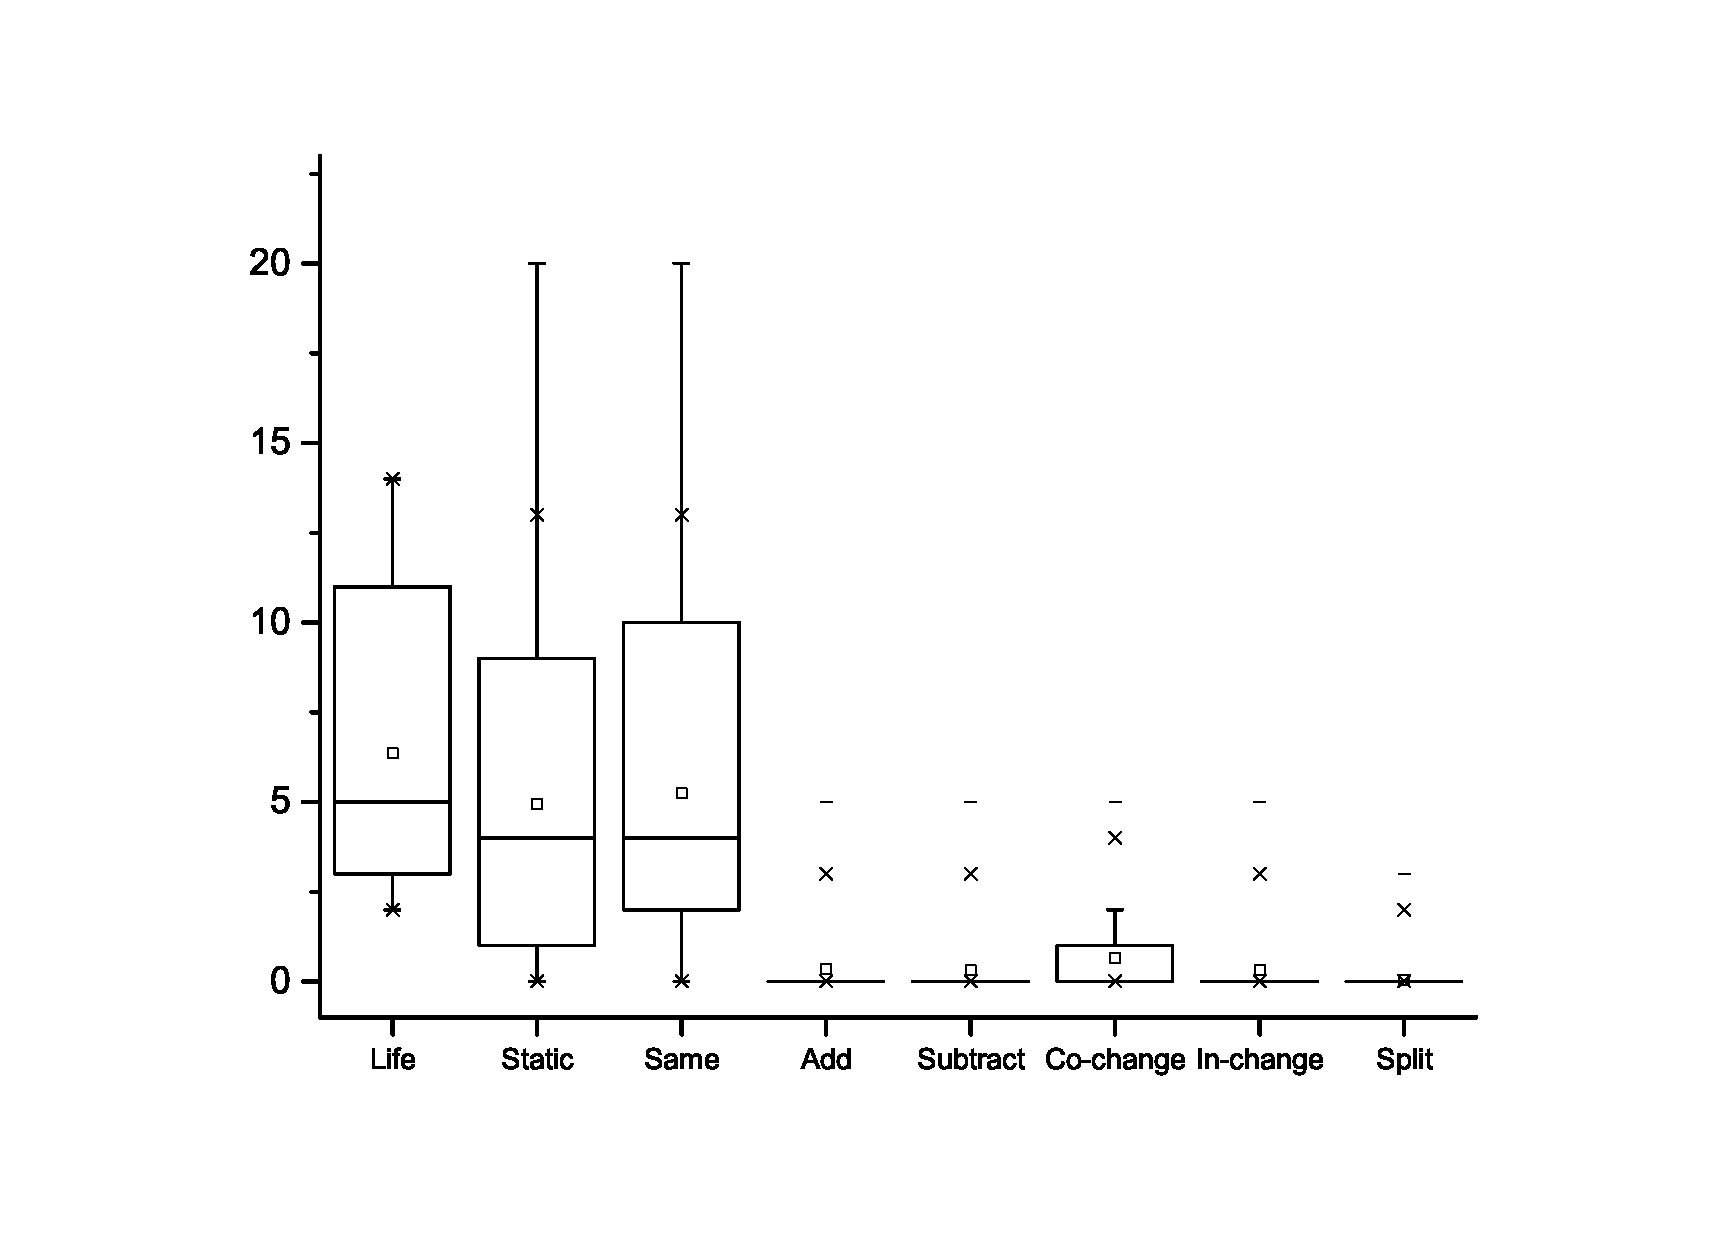
\includegraphics[width=0.85\textwidth]{cgestargo.eps}}}
\subfigure{\label{cgestjedit}}
\addtocounter{subfigure}{-2}
\subfigure[The statistics of clone genealogy evolution for jEdit]
{\subfigure[jEdit中克隆家系的演化模式统计]{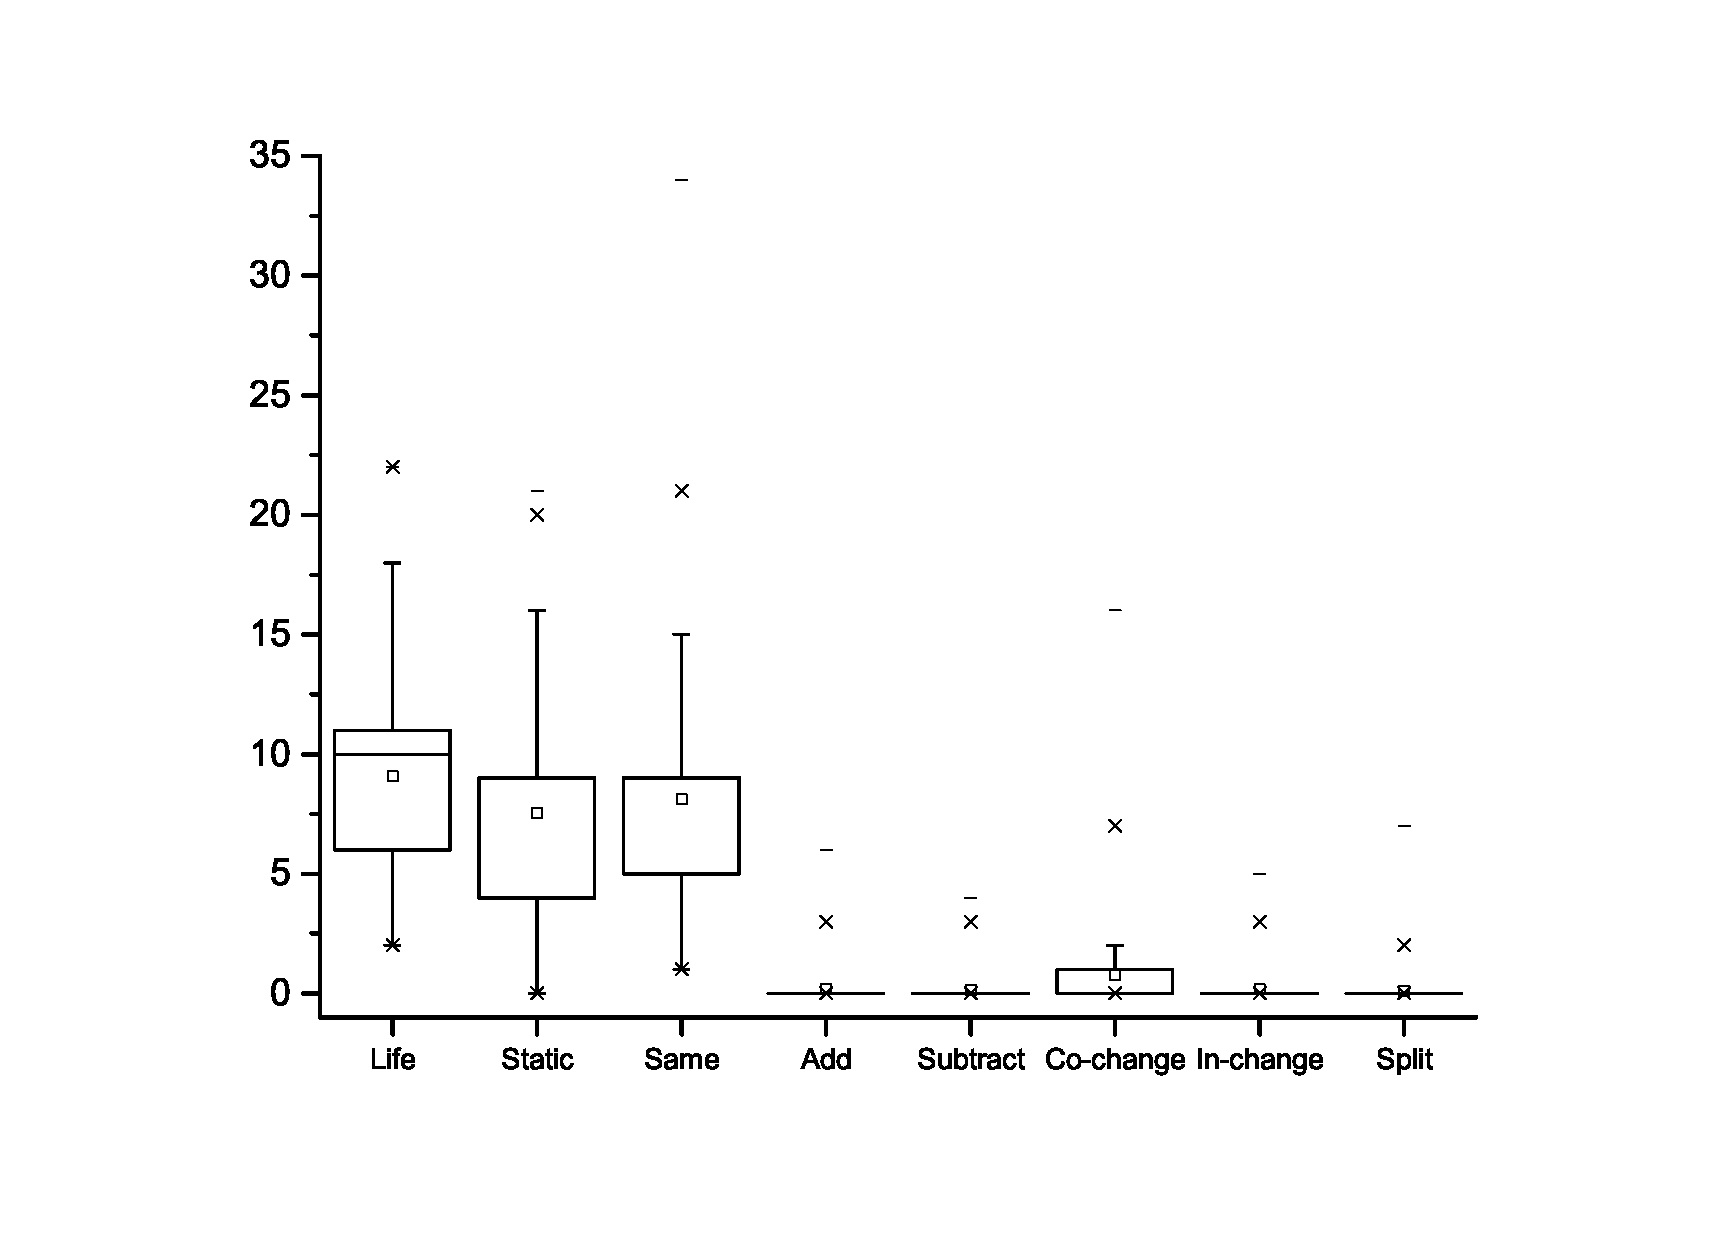
\includegraphics[width=0.85\textwidth]{cgestjedit.eps}}}
\bicaption[cgestas]{}{克隆家系的演化模式统计}
{Fig.$\!$}{The statistics of clone genealogy evolution}
\vspace{-1em}
\end{figure}
 
\BiSubsubsection{克隆家系聚类分析实验}
{Clone Genealogy Experiment of Clustering} 

使用X-means对克隆家系实体的演化情况进行聚类分析(即克隆寿命和克隆演化模式数量),进而挖掘更多的克隆演化特征,结果如表~\ref{cgecluargouml}和~\ref{cgeclujedit}~所示。从表中可以看出,X-means聚类方法将所有克隆家系可以聚类成4个Cluster:Cluster0 - Cluster3。表中第1列给出了四个Cluster的基本情况,分别给出了Cluster中克隆家系的数量和比例。表中第4 - 11列给出了克隆家系每一种属性特征的分布情况,同样使用平均值(Mean)、标准差(SD)和中位数(Median)描述。

表中定义了一个 “Death”的特殊变量,并用其标识实验所收集的克隆家系是否已经死亡。从表中的“Cluster”列和“Death”列中可以发现,所收集的克隆家系是完整的,即大部分的克隆家系仍在演化中并没有死亡。

\begin{table} [h]
\bicaption[cgecluargouml]{}{ArgoUML中克隆家系的聚类结果}
{Table$\!$}{Clustering results of clone genealogy for ArgoUML}
\vspace{0.5em}
\centering
\footnotesize
\begin{tabular}{ccccccccccc}
\toprule[1.5pt]
Cluster&Death&Metric&Life&	Static&	Same&	Add	&Subtract&	Consistent&	Inconsistent&	Split\\ 
\midrule[1pt]
Cluster0&\multirow{3}{*}{5}&Mean	&11.854	&9.795	&10.451	&2.232&	2.232&	3.061&	2.293&	0.390\\ 
82&&SD&1.820&2.989&	3.048&	1.046&	1.081&0.851&1.071&	0.843\\ 
(8\%)&&Median	&11&	10&	10&	2&	2&	3&	2	&0\\ 
%\hline
Cluster1&\multirow{3}{*}{39}&Mean	&10.192&8.831&9.096	&0.171&0.122	&0.444&0.122&0.005\\ 
385&&SD&	1.680	&1.676&1.703&0.398&	0.328	&0.648&	0.328	&0.102\\ 
(37\%)&&Median	&11	&9	&10	&0&	0&	0&	0	&0\\ 
%\hline
Cluster2&\multirow{3}{*}{188}&Mean	&3.294&1.255	&2	&0.471&0.461&1.260	&0.461	&0.010\\
204&&SD&1.228&1.355&1.324&0.639&0.6389&0.440&0.638&0.140\\ 
(20\%)&&Median	&3&	1&	2&	0&	0&	1&	0&	0\\ 
%\hline
Cluster3&\multirow{3}{*}{348}&Mean	&2.795	&1.795	&1.795	&0	&0	&0	&0	&0\\ 
365&&SD&1.081	&1.081&1.081&0	&0	&0	&0	&0\\ 
(35\%)&&Median	&3	&2	&2	&0	&0	&0&	0&	0\\ 
%\hline
All&\multirow{3}{*}{579}&Mean	&6.359&4.936&5.234&0.333	&0.313&0.655	&0.318&0.035\\ 
1036&&SD&4.025	&4.022	&4.062	&0.750	&0.745&0.974&0.757&0.272\\ 
(100\%)&&Median&	5&	4&	4&	0&	0&	0&	0&	0\\
\bottomrule[1.5pt]
\end{tabular}
\end{table} 

\begin{table} [h]
\bicaption[cgeclujedit]{}{jEdit中克隆家系的聚类结果}
{Table$\!$}{Clustering results of clone genealogy for jEdit}
\vspace{0.5em}
\centering
\footnotesize
\begin{tabular}{ccccccccccc}
\toprule[1.5pt]
Cluster&Death&Metric&Life&	Static&	Same&	Add	&Subtract&	Consistent&	Inconsistent&	Split\\
\midrule[1pt]
Cluster0&\multirow{3}{*}{3}&Mean	&19	&15.8	&19.2	&3	&2.3&	6	&2.7&	1.1\\ 
10&&SD&4.830&4.566&	6.426&1.333&	0.949&	4.570&	1.418&2.234\\ 
(4\%)&&Median	&22&	17&	19&	3&	2	&4.5	&2.5&	0\\ 
%\hline
Cluster1&\multirow{3}{*}{35}&Mean	&10.952&	9.445&	9.938&	0.075	&0.075	&0.589&	0.082&	0.041\\ 
146&&SD&2.356&2.166&2.358&0.265	&0.313&	1.074&	0.343&	0.285\\ 
(62\%)&&Median&	10&	9&	9	&0&	0	&0	&0&	0\\ 
%\hline
Cluster2&\multirow{3}{*}{24}&Mean	&6.571&	4.75&	5.607&	0.071&	0.071&	0.857&	0.071&	0.071\\ 
28&&SD&1.168&	1.143&1.227&0.262&0.262&0.970&0.262&0.378\\ 
(12\%)&&Median	&7	&5	&6&	0	&0	&1&	0&	0\\
%\hline
Cluster3&\multirow{3}{*}{48}&Mean	&3.340&	2.132&	2.302&	0.038&	0	&0.208&	0	&0\\ 
53&&SD&	0.732&0.921&0.723&	0.192&	0&	0.454&0	&0\\ 
(22\%)&&Median	&3&	2&	2	&0&	0&	0	&0&	0\\
%\hline
All&\multirow{3}{*}{110}&Mean	&9.072&7.523&	8.110&0.190&	0.152&	0.764	&0.173&	0.080\\ 
237&&SD&4.366&	4.079&4.569&0.690&	0.554&	1.706&0.664	&0.550\\ 
(100\%)&&Median	&10	&9	&9	&0	&0	&0	&0	&0\\
\bottomrule[1.5pt]
\end{tabular}
\end{table} 

为了分析克隆家系的演化情况,非正式给出“稳定的”和“动态的”的克隆家系。如果一个克隆家系中具有大量的稳定的克隆演化模式,即克隆家系中存在大量的“静态(Stactic)”和“相同(Same)”演化模式,则称克隆家系是 “稳定的”克隆家系(Stable Clone Genealogy)。相反地称一个克隆家系是“动态的”克隆家系(Dynamic Clone Genealogy),即该克隆家系具有相对较多的“增加(Add)”,“减少(Subtract)”,“一致/不一致性变化(Consistent/Inconsistent Change)”和“分裂( Split)”模式。

从图~\ref{cgestas}和表~\ref{cgecluargouml}~和~\ref{cgeclujedit}~中,可以很明显的看出,大多数的克隆家系是“稳定的”克隆家系(Cluster1、2、3),并且克隆家系寿命和“稳定的”克隆模式之间存在较强的正相关关系。另一方面,“动态的”克隆家系(Cluster0)数量十分稀少,并且具有较长的寿命且依然存在于系统中。这表明“动态的”克隆演化模式 --- 特别是一致性变化和不一致性变化 --- 通常发生在寿命较长的克隆家系中。因此,软件开发人员应该对动态的克隆家系采取一些必要的措施,因为不一致性的变化可能导致软件缺陷。

对于Cluster3中的克隆家系(表~\ref{cgecluargouml}和~\ref{cgeclujedit}),其寿命较短,并且它们中的大多数已经死亡。但是,这些克隆家系却非常稳定,不存在不一致性变化演化模式。因此可以得出结论:寿命较短的克隆家系比寿命较长的克隆家系更为稳定。这也提醒软件开发人员,不需要关注那些新创建的克隆家系(寿命较短的克隆家系),但随着时间的推移,程序开发人员更应该关注那些依然存在系统中的寿命较长的克隆家系。

综上所述,克隆家系在整个演化过程中大多是稳定的,而较短寿命的克隆家系相比寿命较长的克隆家系更为稳定。 同时,动态的演化模式通常发生在较长寿命的克隆家系中(即使其数量比较稀少),其中一致性变化模式比不一致性变化模式更为频繁。因此,本文建议开发人员应该更加注意寿命较长的克隆家系,并且当克隆代码发生变化时需要考虑同组克隆代码的一致性变化。

%%%%以下是未保留小数的表格
%%%begin{table}[htbp]
%%%\bicaption[cggcluargouml]{}{ArgoUML中克隆家系的聚类结果}
%%%{Table$\!$}{Clone Genealogy Clustering Results of ArgoUML}
%%%\vspace{0.5em}
%%%\centering\wuhao
%%%\begin{tabular}{ccccccccccc}
%%%\toprule[1.5pt]
%%% &Death&&Genealogy Life&	Static&	Same&	Add	&Subtract&	Consistent&	Inconsistent&	Split\\ 
%%%\midrule[1pt]
%%%Cluster0&\multirow{3}{*}{5}&Mean	&11.85366	&9.79268	&10.45122	&2.23171&	2.23171&	3.06098&	2.29268&	0.39024\\ \cline{3-11}
%%%82&&Standard Deviation	&1.81979	&2.98861&	3.04758&	1.04585&	1.08068	&0.85125&1.07138&	0.84263\\ \cline{3-11}
%%%(8\%)&&Median	&11&	10&	10&	2&	2&	3&	2	&0\\ \hline
%%%Cluster1&\multirow{3}{*}{39}&Mean	&10.19221	&8.83117	&9.0961	&0.17143	&0.12208	&0.44416	&0.12208	&0.00519\\ \cline{3-11}
%%%385&&Standard Deviation&	1.67998	&1.67552	&1.70282	&0.39754&	0.3278	&0.64761&	0.3278	&0.10193\\ \cline{3-11}
%%%(37\%)&&Median	&11	&9	&10	&0&	0&	0&	0	&0\\ \hline
%%%Cluster2&\multirow{3}{*}{188}&Mean	&3.29412	&1.2549	&2	&0.47059	&0.46078	&1.2598	&0.46078	&0.0098\\ \cline{3-11}
%%%204&&Standard Deviation	&1.22847	&1.35506	&1.32427	&0.63875	&0.63822	&0.43961	&0.63822	&0.14003\\ \cline{3-11}
%%%(20\%)&&Median	&3&	1&	2&	0&	0&	1&	0&	0\\ \hline
%%%Cluster3&\multirow{3}{*}{348}&Mean	&2.79452	&1.79452	&1.79452	&0	&0	&0	&0	&0\\ \cline{3-11}
%%%365&&Standard Deviation	&1.0813	&1.0813	&1.0813	&0	&0	&0	&0	&0\\ \cline{3-11}
%%%(35\%)&&Median	&3	&2	&2	&0	&0	&0&	0&	0\\ \hline
%%%All&\multirow{3}{*}{579}&Mean	&6.35907	&4.93629	&5.23359	&0.33301	&0.31274	&0.65541	&0.31757	&0.03475\\ \cline{3-11}
%%%1036&&Standard Deviation	&4.02533	&4.0219	&4.06154	&0.74995	&0.74514	&0.97405	&0.75663	&0.27231\\ \cline{3-11}
%%%(100\%)&&Median&	5&	4&	4&	0&	0&	0&	0&	0\\ \hline
%%%\bottomrule[1.5pt]
%%%\end{tabular}
%%%\end{table}

%%%\begin{table}[htbp]
%%%\bicaption[cggclujedit]{}{jEdit中克隆家系的聚类结果}
%%%{Table$\!$}{Clone Genealogy Clustering Results of jEdit}
%%%\vspace{0.5em}
%%%\centering\wuhao
%%%\begin{tabular}{ccccccccccc}
%%%\toprule[1.5pt]
%%%&Death&&Genealogy Life&	Static&	Same&	Add	&Subtract&	Consistent&	Inconsistent&	Split\\
%%%\midrule[1pt]
%%%Cluster0&\multirow{3}{*}{3}&Mean	&19	&15.8	&19.2	&3	&2.3&	6	&2.7&	1.1\\ \cline{3-11}
%%%10&&Standard Deviation	&4.83046	&4.56557&	6.42564	&1.33333&	0.94868&	4.57044&	1.41814	&2.23358\\ \cline{3-11}
%%%(4\%)&&Median	&22&	17&	19&	3&	2	&4.5	&2.5&	0\\ \hline
%%%Cluster1&\multirow{3}{*}{35}&Mean	&10.95205&	9.44521&	9.93836&	0.07534	&0.07534	&0.58904&	0.08219&	0.0411\\ \cline{3-11}
%%%146&&Standard Deviation&2.35572	&2.16566&2.35832	&0.26485	&0.31262&	1.07428&	0.34254&	0.28471\\ \cline{3-11}
%%%(62\%)&&Median&	10&	9&	9	&0&	0	&0	&0&	0\\ \hline
%%%Cluster2&\multirow{3}{*}{24}&Mean	&6.57143&	4.75&	5.60714&	0.07143&	0.07143&	0.85714&	0.07143&	0.07143\\ \cline{3-11}
%%%28&&Standard Deviation	&1.16837&	1.14261	&1.22744	&0.26227&0.26227	&0.97046	&0.26227	&0.37796\\ \cline{3-11}
%%%(12\%)&&Median	&7	&5	&6&	0	&0	&1&	0&	0\\ \hline
%%%Cluster3&\multirow{3}{*}{48}&Mean	&3.33962&	2.13208&	2.30189&	0.03774&	0	&0.20755&	0	&0\\ \cline{3-11}
%%%53&&Standard Deviation&	0.73231	&0.92065	&0.72284&	0.19238&	0&	0.45398	&0	&0\\ \cline{3-11}
%%%(22\%)&&Median	&3&	2&	2	&0&	0&	0	&0&	0\\ \hline
%%%All&\multirow{3}{*}{110}&Mean	&9.07173	&7.52321&	8.1097	&0.18987&	0.1519&	0.76371	&0.173&	0.08017\\ \cline{3-11}
%%%237&&Standard Deviation	&4.36559&	4.07926	&4.56922	&0.6903&	0.55438&	1.70588	&0.66354	&0.55033\\ \cline{3-11}
%%%(100\%)&&Median	&10	&9	&9	&0	&0	&0	&0	&0\\ \hline
%%%\bottomrule[1.5pt]
%%%\end{tabular}
%%%\end{table}

%%%\BiSection{讨论和分析}{Discussion}
%% 
%%%我们的方法取决于NiCad和克隆映射算法构建克隆系谱。 我们使用NiCad检测克隆,其结果然后用于映射克隆,以便构建克隆系谱。更精细的克隆检测工具和更精确的克隆映射算法可能提高后续阶段的质量。请注意,我们的方法很大程度上取决于克隆度量的可用性。我们使用一组指标来表示克隆片段,克隆组,克隆系谱。虽然这些指标对我们有很好的影响,但我们希望将来扩展指标的收集,因为新的有趣指标可以暗示克隆与其进化之间可能存在的新关系。
%%
%%%在将来,我们还可以对具有更多克隆度量的不同软件进行更多的实验。我们相信,我们提出了一些更有意义的结论,以帮助克隆分析和克隆维护。我们还可以对克隆特征进行一些进一步的工作。我们认为克隆特征应该在系统维护期间的克隆分析中使用。例如,我们可以从软件中识别一些特殊的克隆,并且我们打算将其链接到克隆有害性。

\BiSection{本章小结}
{Summary of  this Chapter}
 
为挖掘克隆代码及其演化过程的克隆代码演化特征,本章提出了一种基于X-means聚类的克隆代码演化特征分析方法,为分析克隆代码演化规律提供了有效的手段。本章方法可以分析多版本软件的演化情况,使用聚类分析(X-means)的方法挖掘和分析克隆代码演化特征,帮助程序开发人员理解克隆代码及其演化过程。从克隆片段、克隆组和克隆家系实体三个不同角度,分析和表示克隆代码及其演化情况,并提取相应属性值生成克隆演化特征分析的聚类向量。克隆片段角度重点关注克隆代码的实际变化情况,克隆组角度关注克隆组在相邻两个版本的演化情况,克隆家系则提供了系统中全部克隆代码演化的全局视角。在ArgoUML和jEdit两个软件系统上的实验结果表明:克隆代码在其演化过程中通常是非常稳定的,不会频繁的发生变化。同时,在其演化过程中,仍然存在相当数量的发生变化的克隆代码,需要引起开发人员的关注。在发生变化的克隆代码中,一致性变化的数量多于不一致性变化,因此建议开发人员应在修改克隆代码片段时需要考虑克隆代码的一致性维护问题。本章所挖掘的克隆演化特征,不仅可以帮助开发人员更好地理解克隆,还可以提供一些建议指导开发人员维护系统中克隆代码。本章研究不仅验证了克隆代码一致性维护的必要性,更为本文后续的克隆代码一致性维护需求预测研究奠定了基础。

%本文的创新点如下:
%\begin{itemize}
%\item 
%本文提出了一个框架分析克隆代码的演化特征,可以帮助程序维护人员维护和管理克隆代码。
%\item 
%本文从三个不同的角度视为将克隆代码一种数据进行分析:克隆片段、克隆组和克隆家系,并提取了相应的度量值表示克隆代码。
%\item 
%本文在两个开源系统上进行了实证研究并获得了相关的克隆演化特征,可以帮助理解和维护克隆代码。
%\end{itemize}